\documentclass{article}
\usepackage[utf8]{inputenc}
\usepackage{amssymb}       % Librerías matemáticas
\usepackage{amsthm}        % Definición de teoremas
\usepackage{array}         % Nuevas características a las tablas
\usepackage{bigstrut}      % Líneas horizontales en tablas
\usepackage{bm}            % Caracteres en negrita en ecuaciones
\usepackage{booktabs}      % Permite manejar elementos visuales en tablas
\usepackage{caption}       % Leyendas
\usepackage{changepage}    % Condicionales para administrar páginas
\usepackage{chngcntr}      % Añade números a las leyendas
\usepackage{color}         % Colores
\usepackage{datetime}      % Fechas
\usepackage{enumitem}      % Listas con letras
\usepackage{floatpag}      % Maneja números de páginas
\usepackage{floatrow}      % Permite administrar posiciones en los caption
\usepackage{framed}        % Permite creación de recuadros
\usepackage{gensymb}       % Simbología común
\usepackage{graphicx}      % Propiedades extra para los gráficos
\usepackage{lipsum}        % Permite crear párrafos de prueba
\usepackage{listings}      % Permite añadir código fuente
\usepackage{longtable}     % Permite utilizar tablas en varias hojas
\usepackage{mathtools}     % Permite utilizar notaciones matemáticas
\usepackage{multicol}      % Múltiples columnas
\usepackage{needspace}     % Maneja los espacios en página
\usepackage{pdflscape}     % Modo página horizontal de página
\usepackage{pdfpages}      % Permite administrar páginas en pdf
\usepackage{physics}       % Paquete de matemáticas
% \usepackage{ragged2e}    % Redefine centering
\usepackage{rotating}      % Permite rotación de objetos
\usepackage{selinput}      % Compatibilidad con acentos
\usepackage{setspace}      % Cambia el espacio entre líneas
\usepackage{soul}          % Permite subrayar texto
\usepackage{subfig}        % Permite agrupar imágenes
\usepackage{textcomp}      % Simbología común
\usepackage{url}           % Permite añadir enlaces
\usepackage{wrapfig}       % Posición de imágenes
\usepackage{xspace}        % Adminsitra espacios en párrafos y líneas
\usepackage{amsmath}
%\usepackage{tikz}
\usepackage{mathdots}
\usepackage{yhmath}
\usepackage{cancel}
\usepackage{siunitx}
\usepackage{multirow}
\usepackage{tabularx}
\usepackage[spanish,british]{babel}
\usepackage{hyperref}
\hypersetup{
    colorlinks=true,
    linkcolor=blue,
    filecolor=magenta,      
    urlcolor=cyan
}
%\usetikzlibrary{fadings}
%\usetikzlibrary{patterns}
%\usetikzlibrary{shadows.blur}
%\usetikzlibrary{shapes}


% CONFIG
\newcounter{problemas}[section]
\newcommand{\newpbm}{\stepcounter{problemas}\begin{flushleft}\boxed{\textbf{P.\thesection.\arabic{problemas}}} \hyperlink{S.\thesection.\arabic{problemas}}{Sol} \end{flushleft}}  % Permite crear problema con ajuste de número y sección automático
\newcommand{\np}{\newpbm} % Alias por si prefieres
\newcommand{\sol}[1]{\hypertarget{S.\thesection.#1}{\hspace{1px}}\boxed{\textbf{S.\thesection.#1}}} % Hay que insertar el número de problema a mano, después se podría automatizar/mejorar
\newcommand{\norma}[1]{\abs{\abs{#1}}}
\newcommand{\kte}{4\pi\epsilon_0}

%-\hyperlink{label}{link}
%    -\hypertarget{label}{target}

\title{Apunte Cálculo y Álgebra}
\author{\textit{Le Touffe}}
\date{October 2020}

%----------------
% Comandos útiles
% Letras de esas que denotan conjuntos: \mathbb{}
% Otra fuente de mate-letras (clase C^k): \mathcal{}
%----------------

\begin{document}

\maketitle
\selectlanguage{spanish}
\tableofcontents
\newpage
\chapter{Resultados Útiles}

\section{Identidades}

En esta sección pondremos demostraciones e identidades que son necesarias o útiles para resolver varios problemas.

\subsection{Sumatorias}

\begin{minipage}{0.55\textwidth}
\begin{equation}
\begin{split}
    &\sum^{n}_{k=m} 1 = n - m + 1\\
    &\sum^{n}_{k=m} a_{k} = \sum^{n\pm 1}_{k=m\pm 1} a_{k\mp 1}\\
    &\sum^{n}_{k=m} a_{k} - a_{k+1} = a_{m} - a_{n+1}\\
    &\sum^{n}_{k=0} k = \frac{n(n+1)}{2}\\
\end{split}
\nonumber
\end{equation}
\end{minipage}
\begin{minipage}{0.55\textwidth}
\begin{equation}
\begin{split}
    &\sum^{n}_{k=0} k^{2} = \frac{n(n+1)(2n+1)}{6}\\
    &\sum^{n}_{k=0} k^{3} = {\frac{n(n+1)}{2}}^{2}\\
    &\sum^{n}_{k=0} k\cdot k! = (n+1)! - 1\\
    &\sum^{n}_{k=0} a^{k}b^{n-k} = \frac{a^{n+1}-b^{n+1}}{a-b}\\
\end{split}
\nonumber
\end{equation}
\end{minipage}

\subsection{Límites}

\begin{minipage}{0.55\textwidth}
\begin{equation}
\begin{split}
    & \lim_{x\to 0}\frac{\sin{x}}{x} = 1 \\
    & \lim_{x\to 1}\frac{\ln{x}}{x-1} = 1\\
    & \lim_{x\to 0}\frac{\ln{(x+1)}}{x} = 1\\
    & \lim_{x\to 0}\frac{\tan{x}}{x} = 1\\
    & \lim_{x\to 0}\frac{\arctan{x}}{x} = 1\\
    & \lim_{x\to 0}\frac{x-\ln{(x+1)}}{x^2} = \frac{1}{2}\\
    & \lim_{x\to 0}\frac{\alpha^x-1}{x} = \ln{\alpha}\\
    & \lim_{x\to\infty}\frac{x+\sin{x}}{x-\sin{x}} = 1\\
\end{split}
\nonumber
\end{equation}
\end{minipage}
\begin{minipage}{0.55\textwidth}
\begin{equation}
\begin{split}
    & \lim_{x\to 0}\frac{\arcsin{x}}{x} = 1\\
    & \lim_{x\to 0}\frac{e^x-1}{x} = 1\\
    & \lim_{x\to 0}\frac{(1+x)^{\alpha}-1}{x} = \alpha\\
    & \lim_{x\to 0}\frac{\tan{x}-x}{x^3} = \frac{1}{3}\\
    & \lim_{x\to 0}\frac{1-\cos{x}}{x^2} = \frac{1}{2}\\
    & \lim_{x\to 0}\frac{x-\sin{x}}{x^3} = \frac{1}{6}\\
    & \lim_{x\to 0}\frac{f(a+x)+f(a-x)-2f(a)}{x^2} = f''(a)\\
\end{split}
\nonumber
\end{equation}
\end{minipage}

\subsubsection{Funciones Asintóticamente Equivalentes}

Dadas dos funciones reales $f$ y $h$, se dice que son asintóticamente equivalentes en $a$ si cumplen que

\[\lim_{x\to a}\frac{f(x)}{h(x)} = 1\]

y se nota como $f(x)\sim h(x)(x\to a)$. Al calcular el límite de un producto o cociente de funciones, se puede reemplazar una de ellas por otra asintóticamente equivalente.

\subsubsection{Criterio de Equivalencia Logarítmica}

Dadas dos funciones reales positivas $f$ y $h$, si $\lim_{x\to a}f(x) = 1$, se verifica que

\begin{equation}
\begin{split}
    \lim_{x\to a}f(x)^{h(x)} = e^L &\Leftrightarrow
    \lim_{x\to a}h(x)(f(x)-1) = L\\
    \lim_{x\to a}f(x)^{h(x)} = +\infty &\Leftrightarrow
    \lim_{x\to a}h(x)(f(x)-1) = +\infty\\
    \lim_{x\to a}f(x)^{h(x)} = 0 &\Leftrightarrow
    \lim_{x\to a}h(x)(f(x)-1) = -\infty\\
\end{split}
\nonumber
\end{equation}
\newpage
\subsection{Notación de Landau}

Dadas dos funciones $f, h:A\subseteq E \to F$ tales que

\[\lim_{x\to a}\frac{f(x)}{h(x)} = 0\]

se dice que $f$ es un infinitésimo de orden superior a $h$ en el punto $a$ y se nota como $f = o(h)$.

\subsection{Series de Taylor}

\[\sum^n_{k=0}\frac{f^{(k)}(a)}{k!}(x-a)^k\]

\begin{minipage}{0.55\textwidth}
\begin{equation}
\begin{split}
    & e^x = 1+\sum_{k=1}^n \frac{x^k}{k!} + o(x^n)\\
    & \sin{x} = \sum_{k=1}^n \frac{(-1)^{k+1}}{(2k-1)!}x^{2k+1} +o(x^{2n})\\
    & \cos{x} = \sum_{k=0}^n \frac{(-1)^k}{(2k)!}x^{2k} +o(x^{2n+1})\\
\end{split}
\nonumber
\end{equation}
\end{minipage}
\begin{minipage}{0.55\textwidth}
\begin{equation}
\begin{split}
    & \ln{x+1} = \sum_{k=1}^n \frac{(-1)^{k+1}}{k}x^k +o(x^n)\\
    & \arctan{x} = \sum_{k=1}^n\frac{(-1)^{k+1}}{2k-1}x^{2k-1} +o(x^{2n})\\
    &\arcsin{x} = \sum_{k=1}^n\frac{\prod_{i=1}^k2k-1}{\prod_{i=1}^k2k}
    \frac{x^{2k+1}}{2k+1}+o(x^{2n+2})\\
\end{split}
\nonumber
\end{equation}
\end{minipage}

\subsection{Identidades Trigonométricas}

\begin{minipage}{0.55\textwidth}
\begin{equation}
\begin{split}
    & \sin{x} = \cos{(x-\pi/2)}\\
    & \sin{(a\pm b)} = \sin{a}\sin{b}\pm\cos{a}\cos{b}\\
    & 1+\tan^2{x} = \sec^2{x}\\
    & \sin{(\arccos{x})} = \sqrt{1-x^2}\\
    & \arccos'{x} = \frac{-1}{\sqrt{1-x^2}}\\
    & \tan{x/2} = \frac{1-\cos{x}}{\sin{x}}\\
    & \sin{a}\pm\sin{b} = 2\sin{\frac{a\pm b}{2}}\cos{\frac{a\mp b}{2}}\\
    & \cos{a}-\cos{b} = -2\sin{\frac{a+b}{2}}\sin{\frac{a-b}{2}}\\
    & \sin{a}\cdot\sin{b} = \frac{1}{2}(\cos{(a-b)}-\cos{(a+b)})\\
    & \tan{(a\pm b)}=\frac{\tan{a}\pm\tan{b}}{1\mp \tan{a}\tan{b}}\\
    & \sin{x/2}=\sqrt{\frac{1-\cos{x}}{2}}\\
    & \sin^2{x}=\frac{1-\cos{2x}}{2}\\
    & \sin{(\arctan{x})} = x\sqrt{\frac{1}{1+x^2}}\\
    &\arcsin{x}+\arccos{x}=\frac{\pi}{2}\\
\end{split}
\nonumber
\end{equation}
\end{minipage}
\begin{minipage}{0.55\textwidth}
\begin{equation}
\begin{split}
    & \cos{x} = \sin{(x+\pi/2)}\\
    & \cos{(a\pm b)} = \cos{a}\cos{b}\mp\cos{a}\cos{b}\\
    & 1+\cot^2{x} = \csc^2{x}\\
    & \cos{(\arcsin{x})} = \sqrt{1-x^2}\\
    & \arcsin'{x} = \frac{1}{\sqrt{1-x^2}}\\
    & \tan{x/2} = \frac{\sin{x}}{1+\cos{x}}\\
    & \cos{a}+\cos{b} = 2\cos{\frac{a+b}{2}}\cos{\frac{a-b}{2}}\\
    & \cos{a}\cdot\cos{b} = \frac{1}{2}(\cos{(a+b)}+\cos{(a-b)})\\
    & \sin{a}\cdot\cos{b} = \frac{1}{2}(\sin{(a+b)}+\sin{(a-b)})\\
    & \cos^2{x}+\sin^2{x} = 1\\
    & \cos{x/2}=\sqrt{\frac{1+\cos{x}}{2}}\\
    & \cos^2{x}=\frac{1+\cos{2x}}{2}\\
    & \cos{(\arctan{x})} = \sqrt{\frac{1}{1+x^2}}\\
    & \tan'{x}=1+\tan^2{x}\\
    & \cos^4{x}-\sin^4{x}=\cos{2x}\\
\end{split}
\nonumber
\end{equation}
\end{minipage}

\subsection{Identidades Hiperbólicas}

\begin{minipage}{0.55\textwidth}
\begin{equation}
\begin{split}
    &\sinh{x}=\frac{e^x-e^{-x}}{2}\\
    &\sinh'{x}=\cosh{x}\\
    &\sinh^{-1}{x}=\ln{(x+\sqrt{x^2+1})}\\
    &\sinh{\cosh^{-1}{x}}=\sqrt{x^2-1}\\
    &\frac{d}{dx}(\sinh^{-1}{x})=\frac{1}{\sqrt{x^2+1}}\\
    &\tanh'{x}=1-\tanh^2{x}\\
    &e^x=\cosh{x}+\sinh{x}\\
\end{split}
\nonumber
\end{equation}
\end{minipage}
\begin{minipage}{0.55\textwidth}
\begin{equation}
\begin{split}
    &\cosh{x}=\frac{e^x+e^{-x}}{2}\\
    &\cosh'{x}=\sinh{x}\\
    &\sinh^{-1}{x}=\ln{(x+\sqrt{x^2-1})}\\
    &\sinh{\cosh^{-1}{x}}=\sqrt{x^2-1}\\
    &\frac{d}{dx}(\cosh^{-1}{x})=\frac{1}{\sqrt{x^2-1}}\\
    &\cosh^2{x}-\sinh^2{x}=1\\
    &e^{-x}=\cosh{x}-\sinh{x}\\
\end{split}
\nonumber
\end{equation}
\end{minipage}

\subsection{Números Complejos}

Para $z,w\in\mathbb{C}$ arbitrarios, se verifica que
% No había entendido que te referías a esto exactamente, gracias por agregarlo!
\newline
\begin{minipage}{0.5\textwidth}
\begin{equation}
\begin{split}
    &\overline{z+w}=\Bar{z}+\Bar{w}\\
    &\overline{zw}=\Bar{z}\Bar{w}\\
    &\Bar{z}=z\Leftrightarrow z\in\mathbb{R}\\
    &\Bar{\Bar{z}}=z\\
    &z\Bar{z}=|z|^2\\
    &\mathrm{Re}(z)=\frac{1}{2}(z+\Bar{z})\\
    &\mathrm{Im}(z)=\frac{1}{2i}(z-\Bar{z})\\
    &\mathrm{arg}(\Bar{z}) = 2\pi-\mathrm{arg}(z)\\
    &\mathrm{arg}(zw)=\mathrm{arg}(z)+\mathrm{arg}(w)\,\,
    \mathrm{mod}\,2\pi\\
    &i^i=e^{\frac{-\pi}{2}}
\end{split}
\nonumber
\end{equation}
\end{minipage}

\subsubsection{Raíz de la unidad}

Dados $k\in\mathbb{N}$ y $z \in \mathbb{C}$, se tiene que

\[z^k=1\Leftrightarrow z\in\{e^{\lambda i\frac{2\pi}{k}}\}^{k-1}_{\lambda=0}\]

\newpage
\subsection{Identidades Diferenciales}

Para $F,G$ campos vectoriales, $f,g$ campos escalares, todas de clase $\mathcal{C}^2$, se verifica que

\begin{minipage}{0.55\textwidth}
\begin{equation}
\begin{split}
    &\nabla\cdot(\nabla\times F) = 0\\
    &\nabla\cdot(fF) = f\nabla\cdot F+F\cdot\nabla f\\
    &\nabla\cdot(F\times G) = G\cdot\nabla\times F -
    F\cdot\nabla\times G\\
    &\nabla^2(fg) = f\nabla^2g + 2\nabla f\cdot \nabla g
    + g\nabla^2f\\
    &\nabla^2F=\nabla(\nabla\cdot F)-\nabla\times(\nabla\times F)\\
    &\nabla\times(\nabla f) = 0\\
    &\nabla\times(fF) = f(\nabla\times F)+\nabla f\times F\\\
    &\nabla\cdot(\nabla f\times\nabla g) = 0\\
    &\nabla(f\nabla g- g\nabla f) = f\nabla^2g- g\nabla^2f\\
    &\nabla\times (F\times G) = (\nabla\cdot G)F-
    (\nabla\cdot F)G+(\mathrm{J}F)G-(\mathrm{J}G)F\\
    &\nabla(F\cdot F)=2(\mathrm{J}F)F+2F\times\nabla\times F\\
    &\nabla(F\cdot G)=(\mathrm{J}F)G+(\mathrm{J}G)F
    +F\times\nabla\times G + G\times\nabla\times F\\
    &\nabla (fg) = f\nabla g  + g\nabla f\\
\end{split}
\nonumber
\end{equation}
\end{minipage}

\subsection{Fórmulas Varias}
$\,\,\,\,\,\,$\medbreak
\textbf{Binomio de Newton:}

\[(x+y)^n = \sum^n_{k=0}\frac{n!}{k!(n-k)!}x^{n-k}y^k\]

\bigbreak
\textbf{Desigualdad de las medias:}

\[\left(\prod^n_{i=1}x_i\right)^{\frac{1}{n}}
\leq \frac{1}{n}\sum^n_{i=1}x_i\]

\bigbreak
\textbf{Fórmula de Wallis:}

\[\lim_{n\to\infty}\frac{1}{n}
\left(\frac{\prod^n_{k=1}2k}
{\prod^n_{k=1}2k-1}\right)^2 = \pi\]

\bigbreak
\textbf{Fórmula de Stirling:}

\[\lim_{n\to\infty}\frac{n!e^n}{n^n\sqrt{n}}=\sqrt{2\pi}\]


\newpage
\section{Integrales}

\subsection{Primitivas}
\textit{Se ignora la constante de integración para facilitar la visualización.}\newline
\begin{minipage}{0.55\textwidth}
\begin{equation}
\begin{split}
    &\int\frac{1}{x}dx  = \ln{|x|} \\
    &\int e^{f(x)}f'(x)dx  = e^{f(x)} \\
    &\int \ln{x}dx  = x\ln{x}-x \\
    &\int x\ln{x}dx  = \frac{1}{4}x^2(2\ln{x}-1) \\
    &\int\frac{1}{x^2+a^2}\,dx  = \frac{1}{a}\arctan{\frac{1}{a}}\\
    &\int\frac{1}{\sqrt{x^2-a^2}}\,dx  = \sinh^{-1}{\frac{x}{a}}\\
    &\int\frac{1}{\sqrt{a^2-x^2}}\,dx  = \arcsin{\frac{x}{a}}\\
    &\int \frac{1}{\sqrt{x^2+a^2}}\,dx  = \cosh^{-1}{\frac{x}{a}}\\
    &\int\frac{1}{x\sqrt{x^2-a^2}}\,dx  = \frac{1}{a}\arctan{\left(\frac{\sqrt{x^2-a^2}}{a}\right)}\\
    &\int\frac{1}{x\sqrt{x^2+a^2}}\,dx  = -\frac{1}{a}\ln{\left(\frac{
    a+\sqrt{x^2+a^2}}{x}\right)}\\
    &\int\frac{1}{x\sqrt{a^2-x^2}}\,dx  = -\frac{1}{a}\ln{\left(\frac{a+\sqrt{a^2-x^2}}{x}\right)}\\
    &\int\frac{1}{x^2-a^2}\,dx  = \frac{\ln{|x-a|}-\ln{|x+a|}}{2a}\\
    &\int\frac{1}{a^2-x^2}\,dx  = \frac{\ln{|x+a|}-\ln{|x-a|}}{2a}\\
    &\int\frac{1}{(1+x^2)^2}\,dx  = \frac{x}{2(1+x^2)}+\frac{1}{2}\arctan{x}\\
    &\int\cos{(\ln{x})}\,dx= \frac{x}{2}(\cos{(\ln{x})}+\sin{(\ln{x})})\\
    &\int\sin^4{x}\,dx=\frac{1}{8}\left(\sin{2x}-
\frac{\sin{4x}}{4}-\frac{3x}{2}\right)\\
\end{split}
\nonumber
\end{equation}
\end{minipage}
\begin{minipage}{0.55\textwidth}
\begin{equation}
\begin{split}
    &\int \sin{x}\,dx = -\cos{x} \\
    &\int \cos{x}\,dx = \sin{x} \\
    &\int\tan{x}\,dx  = -\ln{|\cos{x}|} \\
    &\int\sec{x}\,dx  = \ln{|\sec{x}+\tan{x}|}\\
    &\int\csc{x}\,dx  = \ln{|\csc{x}-\cot{x}|}\\
    &\int\tan^2{x}\,dx  = \tan{x}-x \\
    &\int\cot^2{x}\,dx  = -\cot{x}-x \\
    &\int\cos^2{(ax)}\,dx  = \frac{x}{2}+\frac{\sin{(2ax)}}{4a}\\
    &\int\sin^2{(ax)}\,dx  = \frac{x}{2}-\frac{\sin{(2ax)}}{4a}\\
    &\int\cosh^2{(ax)}\,dx  = \frac{x}{2}+\frac{\sinh{(2ax)}}{4a}\\
    &\int\sinh^2{(ax)}\,dx  = \frac{\sinh{(2ax)}}{4a}-\frac{x}{2}\\
    &\int\frac{1}{\cosh{x}}\,dx  = 2\arctan{e^x}\\
    &\int\frac{1}{\sinh{x}}\,dx  = \ln{|e^x-1|}-\ln{|e^x+1|}\\
    &\int\sqrt{a^2-x^2}\,dx  = \frac{x}{2}\sqrt{a^2-x^2}+\frac{a^2}{2}\arcsin{\frac{x}{a}}\\
    &\int\sin{(bx)}e^{ax}\,dx=\frac{a\sin{(bx)}-b\cos{(bx)}}{a^2+b^2}e^{ax}\\
    &\int\frac{x}{\sqrt{a-bx}}\,dx= \frac{-2a}{b^2}\sqrt{a-bx}+\frac{2}{3b^2}(a-bx)^{3/2}\\
    &\int\frac{1}{(a^2+(b-x)^2)^{3/2}}\,dx=\frac{x-b}{a\sqrt{a^2+(b-x)^2}}\\
\end{split}
\nonumber
\end{equation}
\end{minipage}
\newpage
\begin{minipage}{0.55\textwidth}
\begin{equation}
\begin{split}
    &\int|x|\,dx  = \frac{x\abs{x}}{2}\\
    &\int \sin^3{x}\,dx = \frac{1}{4}\left(\frac{\cos{3x}}{3}-3\cos{x}\right)\\
    &\int \cos^3{x}\,dx = \frac{1}{4}\left(\frac{\sin{3x}}{3}+3\sin{x}\right)\\
\end{split}
\nonumber
\end{equation}
\end{minipage}
\begin{minipage}{0.55\textwidth}
\begin{equation}
\begin{split}
    &\int\sqrt{a^2+x^2}\,dx = \frac{x}{2}\sqrt{x^2+a^2}+\frac{a^2}{2}\ln{(x~\sqrt{x^2+a^2})}\\
    &\int\sqrt{x^2-a^2}\,dx = \frac{x}{2}\sqrt{x^2-a^2}-\frac{a^2}{2}\ln{(x+\sqrt{x^2-a^2})}\\
    &\int\frac{x}{(x^2+a^2)^{3/2}}\,dx = -\frac{1}{\sqrt{x^2 + a^2}}\\
\end{split}
\nonumber
\end{equation}
\end{minipage}

\[\int\frac{x}{\sqrt{ax^2 + bx +c}}\,dx = \frac{1}{a}\sqrt{ax^2 +bx +c} - \frac{b}{2a^{3/2}}\ln{\abs{2ax +b+2\sqrt{a(ax^2+bx+c)}}}\]
\bigbreak

\bigbreak
Para funciones de forma $\frac{Ax+B}{ax^2+bx+c}$, se tiene que:

\begin{itemize}
    \item Si $4ac>b^2$
    \[\int\frac{Ax+B}{ax^2+bx+c}\,dx = \frac{A}{2a}\ln{(ax^2+bx+c)}+\frac{2aB-bA}{a\sqrt{4ac-b^2}}\arctan{\left(\frac{2ax+b}{\sqrt{4ac-b^2}}\right)}\]
    \item Si $4ac<b^2$ %este puede que haya que revisarlo
    \[\int\frac{Ax+B}{ax^2+bx+c}\,dx = \frac{1}{2\sqrt{b^2-4ac}}
    \left(\Omega_{-}+\,\Omega_{+}\right)\]
    donde
    \[\Omega_{-} = (2B-A(b-\sqrt{b^2-4ac}))\ln{(2ax+b-\sqrt{b^2-4ac})}\]
    \[\Omega_{+} = (A(b+\sqrt{b^2-4ac})-2B)\ln{(2ax+b+\sqrt{b^2-4ac})}\]
\end{itemize}

\subsection{De Suma a Integral}

Dado un intervalo $[a, b]$ y una partición $\{x_0=a, x_1, x_2, ..., x_n=b\}$ tal que $\Delta x_i = x_{i+1}-x_i$ es una diferencia infinitesimal, considerando $y_i\in [x_i, x_{i+1}]$, por la definición de integral de Riemann, se verifica que

\[\sum f(y_i)\Delta x_i = \int^b_af(x)\,dx\]

Algunos ejemplos son:

\begin{equation}
\begin{split}
    &\lim_{n\to\infty}\frac{1}{n}\sum^n_{k=1}f(k/n)=\int^1_0f(x)\,dx\\
    &\lim_{n\to\infty}\sum^n_{k=1}f(r^{\frac{k}{n}})
    (r^{\frac{k}{n}}-r^{\frac{k-1}{n}})=\int^r_1f(x)\,dx\\
\end{split}
\nonumber
\end{equation}

\subsection{Métodos de Integración}

\subsubsection{Integración por Partes}

Dado que la derivada del producto de dos funciones $f(x)h(x)$ es $f'(x)h(x)+f(x)h'(x)$, la integral de una función de forma $f'(x)h(x)$ se puede calcular como

\[\int f'(x)h(x)\,dx = f(x)h(x) - \int f(x)h'(x)\,dx\]

\subsubsection{Cambio de Variable}

Sean $h \in \mathcal{C}^1$, $f\in\mathcal{C}^0$, $F$ una primitiva de $f$ y $H = F \circ h$, se verifica que

\[\int^b_af(h)h'=H(b)-H(a)=F(h(b))-F(h(a))=\int^{h(b)}_{h(a)}f\]

esto es un cambio de variable. Hay dos formas de notarlo:

\begin{equation}
\begin{split}
    &\int^{h(b)}_{h(a)}f(x)\,dx =
    \begin{bmatrix}
    x = h(t)\\
    dx= h'(t)dt
    \end{bmatrix} = \int^b_af(h(t))h'(t)\,dt\\
    &\int^b_af(h(t))h'(t)\,dt = \int^{h(b)}_{h(a)} f(h)\,dh\\
\end{split}
\nonumber
\end{equation}

La segunda forma es especialmente útil para ecuaciones diferenciales.

\subsubsection{F(sin x, cos x)}

Cuando se tiene integrales de forma

\[\int F(\sin{x}, \cos{x})\,dx\]

puede convenir utilizar el cambio de variable $x = 2\arctan{t}$, para el cual se cumple que

\begin{minipage}{0.55\textwidth}
\begin{equation}
    \sin{x}=\frac{2t}{1+t^2}\,\,\,\,\,\,\,\,
    \cos{x}=\frac{1-t^2}{1+t^2}\,\,\,\,\,\,\,\,
    t=\tan{\frac{x}{2}}\,\,\,\,\,\,\,\,
    dx=\frac{2}{1+t^2}dt
\nonumber
\end{equation}
\end{minipage}

\[\int F(\sin{x}, \cos{x})\,dx = 
\begin{bmatrix}
x = 2\arctan{t}\\
dx=\frac{2}{1+t^2}dt
\end{bmatrix}
= \int F\left(\frac{2t}{1+t^2},\frac{1-t^2}{1+t^2}\right)
\frac{2}{1+t^2}\,dt\]

Casos particulares:

\begin{itemize}
    \item si $F(-\sin{x}, \cos{x}) = -F(\sin{x}, \cos{x})$, el cambio $t = \cos{x}$ puede funcionar.
    \item si $F(\sin{x}, -\cos{x}) = -F(\sin{x}, \cos{x})$, el cambio $t = \sin{x}$ puede funcionar.
    \item si $F(-\sin{x}, -\cos{x}) = F(\sin{x}, \cos{x})$, el cambio $t = \tan{x}$ puede funcionar.
\end{itemize}

\subsubsection{Potencias Racionales}

Sea $L(x) = \frac{ax+b}{cx+d}$ tal que $ad-bc\neq 0$, para integrales del tipo

\[\int F(x, L(x)^{r_1}, L(x)^{r_2}, ..., L(x)^{r_n})\,dx\]

donde $r_1, r_2, ..., r_n \in \mathbb{Q}$, tomando $q$ como el mínimo común denominador de $\{r_i\}_{i=1}^n$, se puede hacer el cambio de variable

\begin{equation}
\begin{split}
\int F(x, L(x)^{r_1}, L(x)^{r_2}, ..., L(x)^{r_n})\,dx & =
\begin{bmatrix}
x = L^{-1}(t^q) = P(t)\\
dx=P'(t)dt
\end{bmatrix}\\ & =
\int F(P(t), t^{qr_1}, t^{qr_2}, ..., t^{qr_n})P'(t)\,dt
\end{split}
\nonumber
\end{equation}

\subsubsection{Integrales Binomias}

Se llama integral binomia a aquellas de forma

\[\int x^\alpha(a+bx^\beta)^\gamma\,dx\]

donde $\alpha, \beta, \gamma \in \mathbb{Q}\setminus\{0\}$ y $a, b\in\mathbb{R}\setminus\{0\}$. Tomando $r = \frac{\alpha+1}{\beta}-1$, se puede hacer el cambio de variable

\[\int x^\alpha(a+bx^\beta)^\gamma\,dx =
\begin{bmatrix}
x = t^\frac{1}{\beta}\\
dx=\frac{1}{\beta}t^{\frac{1}{\beta}-1}dt
\end{bmatrix}
= \frac{1}{\beta}\int t^r(a+bt)^\gamma\,dt\]

Esta integral es del tipo que considera el método de potencias racionales si 

\begin{itemize}
    \item $\gamma\in\mathbb{Z}$, siendo de forma $\int F(t, t^r)dt$
    \item $r\in\mathbb{Z}$, siendo de forma $\int F(t, (a+bt)^\gamma)dt$
    \item $r+\gamma\in\mathbb{Z}$, siendo de forma $\int \left(\frac{a+bt}{t}\right)^\gamma t^{r+\gamma}dt$
\end{itemize}

\subsubsection{Raíces de Parábolas}

Para integrales de forma

\[\int F(x, \sqrt{ax^2+bx+c})\, dx\]

Si $\alpha, \beta\in\mathbb{R}$ son raíces de $ax^2+bx+c$, se verifica que

\[\sqrt{ax^2+bx+c}=\sqrt{a(x-\alpha)(x-\beta)} =
(x-\alpha)\sqrt{\frac{a(x-\beta)}{x-\alpha}}\]

por lo que conviene hacer el cambio

\begin{equation}
\int F(x,\sqrt{ax^2+bx+c})\,dx =
\begin{bmatrix}
x = \frac{\alpha t^2-a\beta}{t^2-a} = r(t)\\
dx = r'(t)dt
\end{bmatrix} =
\int F(r(t),(r(t)-\alpha)t)r'(t)\,dt
\nonumber
\end{equation}
\bigbreak
\bigbreak
Si $ax^2+bx+c$ no tiene raíces reales y $c>0$, se puede hacer el cambio

\begin{equation}
\int F(x,\sqrt{ax^2+bx+c})\,dx =
\begin{bmatrix}
x = \frac{b-2t\sqrt{c}}{t^2-a} = r(t)\\
dx = r'(t)dt
\end{bmatrix} =
\int F(r(t),tr(t)+\sqrt{c})r'(t)\,dt
\nonumber
\end{equation}
\bigbreak
donde $tx+\sqrt{c} = \sqrt{ax^2+bx+c}$

\subsection{Identidades con Integrales}

\begin{minipage}{0.5\textwidth}
\begin{equation}
\begin{split}
    &\int^{2\pi}_0\cos^m\theta\sin^n\theta\,d\theta=
    \frac{n-1}{m+n}\int^{2\pi}_0\cos^m\theta
    \sin^{n-2}\theta\,d\theta\\
    &\int^{2\pi}_0\cos^m\theta\,d\theta=\frac{m-1}{m}
    \int^{2\pi}_0\cos^{m-2}\theta\,d\theta\\
    &I_n=\int x^{2n-1}e^{x^2}\,dx\Rightarrow I_{n+1}=
    \frac{x^{2n}e^{x^2}-2nI_n}{2}\\
    &\int^{+\infty}_0 e^{-\alpha x}\,dx=\frac{1}{\alpha}\\
    &\int^{+\infty}_{-\infty}e^{x^2}\,dx=\sqrt{\pi}\\
\end{split}
\nonumber
\end{equation}
\end{minipage}

\newpage
\section{Sistemas de Coordenadas}

\subsection{Cilíndricas}

\[\Vec{r}(\rho,\phi,z)\]

\begin{figure}[H]
    \centering
    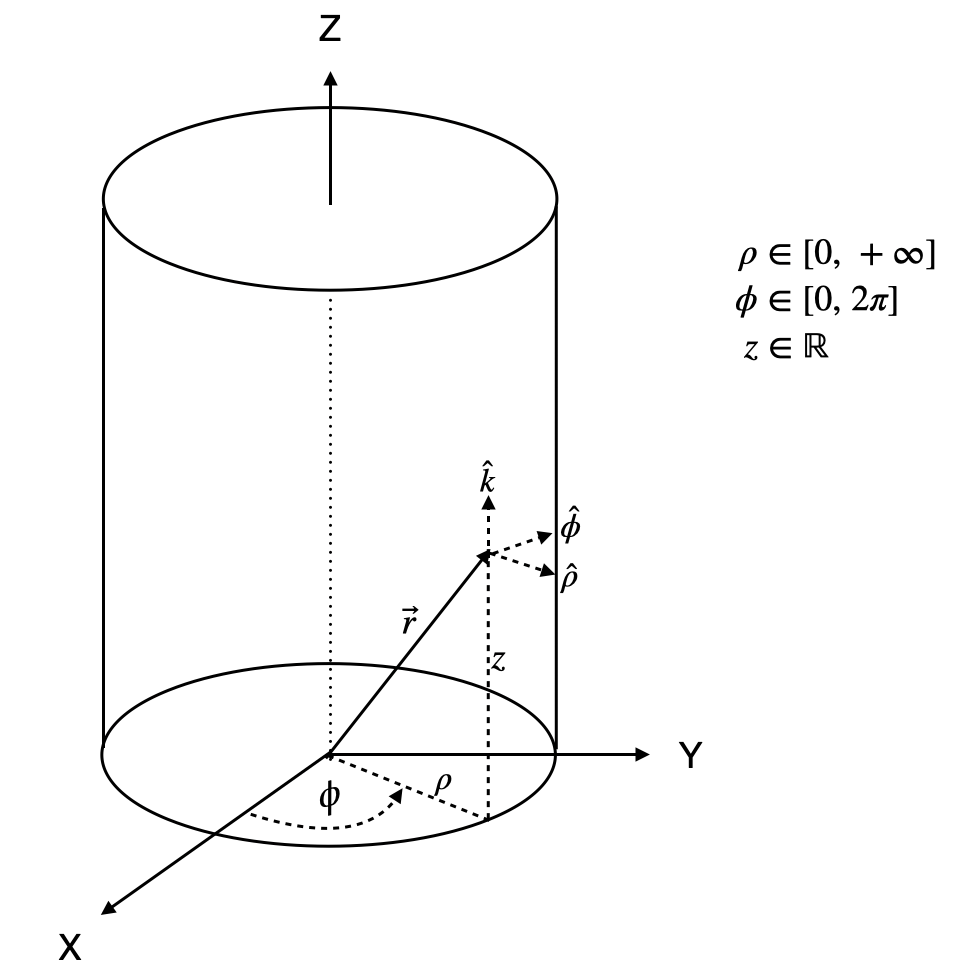
\includegraphics[width=0.45\textwidth]{Resultados Útiles/imgs/coords_cilind_DFI.png}
    \caption{Coordenadas cilíndricas en el plano cartesiano}
    \label{fig:C.cilindricas}
\end{figure}

\begin{minipage}{0.55\textwidth}
\begin{equation}
\begin{split}
    &x = \rho\cos{\phi}\\
    &y = \rho\sin{\phi}\\
\end{split}
\nonumber
\end{equation}
\end{minipage}
\begin{minipage}{0.35\textwidth}
\begin{equation}
\begin{split}
    & \rho = \sqrt{x^2+y^2}\\
    & \phi = \arctan{\frac{y}{x}}\\
\end{split}
\nonumber
\end{equation}
\end{minipage}

\bigbreak
Factores escalares:
\begin{itemize}
    \item $h_\rho = 1$
    \item $h_\phi = \rho$
    \item $h_z = 1$
\end{itemize}

Vectores unitarios:

\begin{itemize}
    \item $\hat{\rho} = \cos{\phi}\,\hat{x}+\sin{\phi}\,\hat{y}$
    \item $\hat{\phi} = -\sin{\phi}\,\hat{x}+\cos{\phi}\,\hat{y}$
    \item $\hat{x}=
    \cos{\phi}\,\hat{\rho}-\sin{\phi}\,\hat{\phi}$
    \item $\hat{y}=
    \sin{\phi}\,\hat{\rho}+\cos{\phi}\,\hat{\phi}$
\end{itemize}

\medbreak

Gradiente:

\[\nabla F = \frac{\partial F}{\partial \rho}\hat{\rho} + \frac{1}{\rho}\frac{\partial F}{\partial \phi}\hat{\phi} + \frac{\partial F}{\partial z}\hat{z}\]

Divergencia:

\[\nabla \cdot \vec{F} = \frac{1}{\rho}\left(\frac{\partial(F_{\rho}\rho)}{\partial\rho}+\frac{\partial F_{\phi}}{\partial\phi}+\frac{\partial(F_{z}\rho)}{\partial z}\right)\]

Rotor:
% Elimine un rho que acompañaba a dF_phi/dphi
\[\nabla\times\vec{F} = \frac{1}{\rho}\left(\frac{\partial F_{z}}{\partial \phi}-\rho\frac{\partial F_{\phi}}{\partial z}\right)\hat{\rho} + \left(\frac{\partial F_{\rho}}{\partial z}-\frac{\partial F_{z}}{\partial \rho}\right)\hat{\phi} + \frac{1}{\rho}\left(\frac{\partial(F_{\phi}\rho)}{\partial \rho}-\frac{\partial F_{\rho}}{\partial \phi}\right)\hat{z}\]

\medbreak

Diferenciales:

\begin{itemize}
    \item Linea:
    \[d\vec{r} = d\rho\hat{\rho} + \rho d\phi\hat{\phi}+dz\hat{z}\]
    \item Superficie:
    \[d\vec{S} = \rho\,d\phi dz\hat{\rho}+d\rho dz\hat{\phi}+\rho\, d\rho d\phi\hat{z}\]
    \item Volumen:
    \[dV = \rho\,d\rho d\phi dz\]
\end{itemize}

\newpage
%%%%%%%%%%%%%%%%%%%%%%%%%%%%%%%%%%%%%%%%%%%%%%%%%%%%%%
\subsection{Esféricas}

\[\Vec{r}(r,\phi,\theta)\]

\begin{figure}[H]
    \centering
    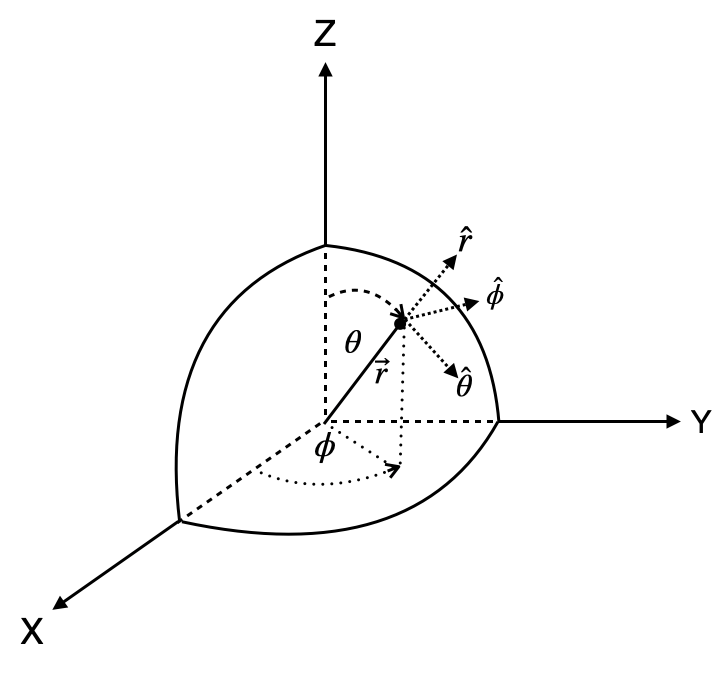
\includegraphics[width=0.5\textwidth]{Resultados Útiles/imgs/coords_esferc_DFI.png}
    \caption{Coordenadas esféricas en el plano cartesiano}
    \label{fig:C.esfericas}
\end{figure}

\begin{minipage}{0.55\textwidth}
\begin{equation}
\begin{split}
    &x = r\sin{\theta}\cos{\phi}\\
    &y = r\sin{\theta}\sin{\phi}\\
    &z = r\cos{\theta}\\
\end{split}
\nonumber
\end{equation}
\end{minipage}
\begin{minipage}{0.35\textwidth}
\begin{equation}
\begin{split}
    & r = \sqrt{x^2+y^2+z^2}\\
    & \phi = \arctan{\frac{y}{x}}\\
    & \theta = \arctan{\left(\frac{\sqrt{x^2+ y^2}}{z}\right)}
\end{split}
\nonumber
\end{equation}
\end{minipage}

\bigbreak
Factores escalares:
\begin{itemize}
    \item $h_r = 1$
    \item $h_\phi = r\sin{\theta}$
    \item $h_\theta = r$
\end{itemize}
\bigbreak
Vectores unitarios:

\begin{itemize}
    \item $\hat{r} = \sin(\theta)\cos(\phi)\hat{x} + \sin(\theta)\sin(\phi)\hat{y} + cos(\theta)\hat{z}$
    \item $\hat{\phi} = -\sin(\phi)\hat{x}+\cos(\phi)\hat{y}$
    \item $\hat{\theta} = \cos(\theta)cos(\phi)\hat{x} + \cos(\theta)\sin(\phi)\hat{y}-\sin(\theta)\hat{z}$
    \item $\hat{x}=\sin{(\theta)\cos{(\phi)}}\hat{r}-\sin{(\phi)}\hat{\phi}+\cos{(\theta)}\cos{(\phi)}\hat{\theta}$
    \item $\hat{y}=\sin{(\theta)\sin{(\phi)}}\hat{r}+\cos{(\phi)}\hat{\phi}+\cos{(\theta)}\sin{(\phi)}\hat{\theta}$
    \item $\hat{z}=\cos{(\theta)}\hat{r}-\sin{(\theta)}\hat{\theta}$
\end{itemize}

\bigbreak

Gradiente:

\[\nabla F = \frac{\partial F}{\partial r}\hat{r} + \frac{1}{rsin(\theta)}\frac{\partial F}{\partial \phi}\hat{\phi} + \frac{1}{r}\frac{\partial F}{\partial \theta}\hat{\theta}\]

Divergencia:

\[\nabla \cdot \vec{F} = \frac{1}{r^2sin(\theta)}\left(\frac{\partial(F_{r}r^2sin(\theta))}{\partial r}+\frac{\partial (F_{\phi}r)}{\partial\phi}+\frac{\partial(F_{\theta}rsin(\theta))}{\partial \theta}\right)\]

Rotor:

\[\nabla\times\vec{F} = \frac{1}{r\sin\theta} \left( \frac{\partial}{\partial \theta} \left(F_\phi\sin\theta \right) - \frac{\partial F_\theta}{\partial \phi} \right) \hat{r} + \frac{1}{r} \left( \frac{1}{\sin\theta} \frac{\partial F_r}{\partial \phi} - \frac{\partial}{\partial r} \left( r F_\phi \right) \right) \hat{\theta} + \frac{1}{r} \left( \frac{\partial}{\partial r} \left( r F_{\theta} \right) - \frac{\partial F_r}{\partial \theta} \right) \hat{\phi}\]

Diferenciales:

\begin{itemize}
    \item Linea:
    \[d\vec{r} = dr\hat{r} + r\sin(\theta)\, d\phi\hat{\phi}+r\,d\theta\hat{\theta}\]
    \item Superficie:
    \[d\vec{S} = r^2\sin(\theta)\,d\phi d\theta\hat{r}+r\,drd\theta\hat{\phi}+r\sin(\theta)\,dr d\phi\hat{\theta}\]
    \item Volumen:
    \[dV = r^2\sin(\theta)\,dr d\phi d\theta\]
\end{itemize}

\newpage
%%%%%%%%%%%%%%%%%%%%%%%%%%%%%%%%%%%%%%%%%%%%%%%%%%%%%%%%%%%%%
\subsection{Parabólicas}

\[\Vec{r}(\epsilon,\eta,\phi)\]

\begin{minipage}{0.55\textwidth}
\begin{equation}
\begin{split}
    &x = \epsilon\eta\cos{\phi}\\
    &y = \epsilon\eta\sin{\phi}\\
    &z = \frac{1}{2}(\eta^2-\epsilon^2)\\
\end{split}
\nonumber
\end{equation}
\end{minipage}
\begin{minipage}{0.35\textwidth}
\begin{equation}
\begin{split}
    & \epsilon = \sqrt{x^2+y^2+z^2}-z\\
    & \eta = \sqrt{x^2+y^2+z^2}+z\\
    & \phi = \arctan{\left(\frac{y}{x}\right)}
\end{split}
\nonumber
\end{equation}
\end{minipage}

\bigbreak
Factores escalares:
\begin{itemize}
    \item $h_\epsilon = \sqrt{\epsilon^2+\eta^2}$
    \item $h_\eta = \sqrt{\epsilon^2+\eta^2}$
    \item $h_\phi = \epsilon\eta$
\end{itemize}
\bigbreak
Vectores unitarios:

\begin{itemize}
    \item $\hat{\epsilon} = \frac{1}{\sqrt{\epsilon^2+\eta^2}}(\eta(\cos{\phi}\,\hat{x}+\sin{\phi}\,\hat{y})-\epsilon\hat{z})$
    \item $\hat{\eta} =  \frac{1}{\sqrt{\epsilon^2+\eta^2}}(\epsilon(\cos{\phi}\,\hat{x}+\sin{\phi}\,\hat{y})+\eta\hat{z})$
    \item $\hat{\phi} = -\sin{\phi}\,\hat{x}+\cos{\phi}\,\hat{y}$
\end{itemize}

\bigbreak

Gradiente:

\[\nabla F = \frac{1}{\sqrt{\epsilon^2+\eta^2}}\frac{\partial
 f}{\partial \epsilon}\hat{\epsilon}+\frac{1}{\sqrt{\epsilon^2+\eta^2}}\frac{\partial
 f}{\partial \eta}\hat{\eta}+\frac{1}{\epsilon\eta}\frac{\partial f}{\partial \phi}\hat{\phi}\]

Divergencia:

\[\nabla \cdot \vec{F} = \frac{1}{\epsilon\eta(\epsilon^2+\eta^2)}
\left(
\frac{\partial(F_\epsilon\epsilon\eta\sqrt{\epsilon^2+\eta^2})}{\partial\epsilon}+
\frac{\partial(F_\eta\epsilon\eta\sqrt{\epsilon^2+\eta^2})}{\partial\eta}+(\epsilon^2+\eta^2)
\frac{\partial F_\phi}{\partial\phi}\right)\]

Rotor:

\[\left(\nabla\times\vec{F}\right)_\epsilon =
\frac{1}{\epsilon\eta\sqrt{\epsilon^2+\eta^2}}
\left(\epsilon
\frac{\partial(F_\phi\eta)}{\partial\eta}-\sqrt{\epsilon^2+\eta^2}\frac{\partial F_\eta}{\partial\phi}\right)\]
\[\left(\nabla\times\vec{F}\right)_\eta=\frac{1}{\epsilon\eta\sqrt{\epsilon^2+\eta^2}}
\left(\sqrt{\epsilon^2+\eta^2}
\frac{\partial F_\epsilon}{\partial\phi}-\eta
\frac{\partial(F_\phi\epsilon)}{\partial\epsilon}\right)\]
\[\left(\nabla\times\vec{F}\right)_\phi=
\frac{1}{\epsilon^2+\eta^2}
\left(\frac{\partial(F_\eta\sqrt{\epsilon^2+\eta^2})}{\partial\epsilon}-\frac{\partial(F_\epsilon\sqrt{\epsilon^2+\eta^2})}{\partial\eta}\right)\]
\newpage
Diferenciales:

\begin{itemize}
    \item Linea:
    \[d\vec{r} = \sqrt{\epsilon^2+\eta^2}d\epsilon\,\hat{\epsilon} + \sqrt{\epsilon^2+\eta^2}d\eta\,\hat{\eta}+\epsilon\eta d\phi\,\hat{\phi}\]
    \item Superficie:
    \[d\vec{S} = \epsilon\eta\sqrt{\epsilon^2+\eta^2}\,d\eta d\phi\hat{\epsilon}+\epsilon\eta\sqrt{\epsilon^2+\eta^2}\,d\phi d\epsilon\hat{\eta}+(\epsilon^2+\eta^2)\,d\epsilon d\eta\hat{\phi}\]
    \item Volumen:
    \[dV = \epsilon\eta(\epsilon^2+\eta^2)\,d\epsilon d\eta d\phi\]
\end{itemize}

\subsection{Elípticas 1}

\[\Vec{r}(\mu,\theta,z)\]

\begin{minipage}{0.55\textwidth}
\begin{equation}
    x = a\cosh{\mu}\cos{\theta}\,\,\,\,\,\,\,\,
    y = a\sinh{\mu}\sin{\theta}
\nonumber
\end{equation}
\end{minipage}

\bigbreak
Factores escalares:
\begin{itemize}
    \item $h_\mu = a\sqrt{\cosh^2{\mu}\cos^2{\theta}
    +\sinh^2{\mu}\sin^2{\theta}}$
    \item $h_\theta = a\sqrt{\cosh^2{\mu}\cos^2{\theta}
    +\sinh^2{\mu}\sin^2{\theta}}$
\end{itemize}
\bigbreak
Vectores unitarios:

\begin{itemize}
    \item $\hat{\mu}=\frac{\sinh{\mu}\cos{\theta}\hat{x}+\cosh{\mu}\sin{\theta}\hat{y}}{\sqrt{\cosh^2{\mu}\cos^2{\theta}
    +\sinh^2{\mu}\sin^2{\theta}}}$
    \item $\hat{\theta}=\frac{-\cosh{\mu}\sin{\theta}\hat{x}+\sinh{\mu}\cos{\theta}\hat{y}}{\sqrt{\cosh^2{\mu}\cos^2{\theta}+\sinh^2{\mu}\sin^2{\theta}}}$
\end{itemize}

\bigbreak

%Gradiente:



%Divergencia:



%Rotor:



%Diferenciales:

%\begin{itemize}
%    \item Linea:
    
%    \item Superficie:
    
%    \item Volumen:
    
%\end{itemize}

\newpage
\section{Teoremas}

En este apartado van los teoremas que no encajan en el resto de secciones

\subsection{Teorema de Taylor-Young}
\label{T:Taylor-Young}
Sean $f:A\subseteq \mathbb{R} \to \mathbb{R}$ una función $n$-veces derivable en $a\in A$ y $T_n(f,a)$ el polinomio de Taylor de orden $n$ de $f$ en $a$, se verifica que

\[f(x)-T_n(f,a)=o(x-a)^n\]

Como consecuencia de esto, al calcular ciertos límites en $a$, se puede reemplazar $\frac{f(x)}{(x-a)^n}$ por $\frac{T_n(f,a)}{(x-a)^n}$. Además, si $f$ es $n+1$ veces derivable se cumple que

\[\lim_{x\to a}\frac{f(x)-T_n(f,a)}{(x-a)^{n+1}}=\frac{f^{n+1}(a)}{(n+1)!}\]

\newpage
%\input{Lineal/Matrices1}
%\input{Lineal/Espacios Vectoriales}
%\input{Lineal/Transformaciones Lineales}
%\input{Lineal/Matrices2}
%\input{Lineal/Ortogonalidad}
%\input{Lineal/Matrices3}
%\chapter{Ecuaciones Diferenciales Ordinarias}

Sea $y: A\subseteq\mathbb{R}\to\mathbb{R}$ una función de clase $\mathcal{C}^n$, se define una EDO como la identidad

\[F(x, y(x),y'(x),...,y^{(n)}(x))=0\]

donde $x\in A$ es una variable arbitraria e $y$ es la incógnita.

\begin{itemize}
    \item \textbf{Orden:} El orden de una EDO es el nivel máximo de derivación de $y$.
    \item\textbf{Grado:} El grado de una EDO es el exponente del término que determina el orden.
\end{itemize}

\section{EDO Lineal}

Se denomina EDO lineal de orden $n$ a aquellas de forma

\[\sum^n_{k=0}a_k(x)y^{(n)}=Q(x)\]

A las funciones $\{a_k\}^n_{k=0}$ se les llama coeficientes y a $Q$ lado derecho. Si el lado derecho es nulo se dice que la EDO es homogénea.

\subsection{Principio de Superposición}

Sea $L(y)$ un \encuote{polinomio diferencial}

\[L(y)=\sum^n_{k=0}a_ky^{(k)}\]

el principio de superposición indica que si para $y_1,y_2\in \mathcal{C}^n$

\[L(y_1)=P_1(x)\]
\[L(y_2)=P_2(x)\]

entonces se verifica que

\[L(y_1+y_2) = L(y_1) + L(y_2) = P_1(x)+P_2(x)\]

$L$ es una transformación lineal. Con esto, el kernel de $L$ 

\[\mathcal{H} = \mathrm{ker}(L) = \{y_h\in\mathcal{C}^n\,|\,L(y_h)=0\}\]

define el subespacio vectorial de las soluciones de la EDO homogénea

\[\sum^n_{k=0}a_ky^{(k)}=0\]

\subsection{EDO no Lineal}

\textbf{\textit{Una EDO no lineal es una EDO que no es lineal}}


\newpage
%\input{EDO/Lineales}
%\input{EDO/Transformada}
%\input{EDO/Sistemas}
\section{Cálculo en Varias Variables}

\subsection{Función en Varias Variables}

Sean $\mathbf{E}, \mathbf{F}$ espacios vectoriales arbitrarios, se definen las funciones en varias variables como aquellas de forma

\[f: A\subseteq\mathbf{E}\to B\subseteq\mathbf{F}\]

En adelante usaremos $\mathbf{E}$ y $\mathbf{F}$ para referirnos a espacios vectoriales.

\subsection{Normas}

Dado $\mathbf{E}$ un espacio vectorial sobre $\mathbb{R}$, se dice que $N:\mathbf{E}\to\mathbb{R}$ es una norma de $\mathbf{E}$ si cumple que

\begin{itemize}
    \item $\forall x\in\mathbf{E}:\, N(x)\geq 0$
    \item $\forall x\in\mathbf{E}:\, N(x)=0\Leftrightarrow
    x=0$
    \item $\forall\lambda\in\mathbb{R}\forall x\in\mathbf{E}:\,
    N(\lambda x) = |\lambda | N(x)$
    \item $\forall x,y\in\mathbf{E}:\, N(x+y)\leq N(x)+N(y)$
\end{itemize}

En tal caso se llama a $\mathbf{E}$ un espacio normado. Se suele usar $\|\cdot\|_\infty$ para notar las normas definidas por supremos

\subsubsection{Normas en $\mathbb{R}^n$}

\begin{itemize}
    \item $\|x\|_p=\left(\sum^n_{i=1}|x_i|^p\right)^{\frac{1}{p}}$
    \item $\|x\|_\infty = \max\{|x_i|\}^n_{i=1}$
\end{itemize}

\subsubsection{Normas Equivalentes}

Dos normas $\|\cdot\|_a$ y $\|\cdot\|_b$ de un mismo espacio vectorial $\mathbf{E}$ son equivalentes si se cumple que

\[\exists L_a, L_b\in\mathbb{R}^+\,\forall x\in\mathbf{E}
:\, \|x\|_a \leq L_a\|x\|_b \wedge \|x\|_b \leq L_b\|x\|_a\]

Todas las normas en $\mathbb{R}^n$ son equivalentes.

\subsection{Bolas}

Sean $\mathbf{E}$ un espacio normado, $a\in\mathbf{E}$ y $r\in\mathbb{R}^+$, se definen

\begin{itemize}
    \item \textbf{Bola Abierta}: $B(a,r)=\{x\in\mathbf{E}\,
    |\,\|x-a\|<r\}$
    \item \textbf{Bola Cerrada}: $\bar{B}(a,r)=\{x\in\mathbf{E}\,|\,\|x-a\|<r\}$
\end{itemize}

Para $B_a$ y $B_b$ bolas definidas en un mismo espacio con normas equivalentes, se verifica que

\[\forall\varepsilon\in\mathbb{R}^+
\exists\delta\in\mathbb{R}^+:\,B_a(c,\delta)\subseteq B_b(c,\varepsilon)\]
\[\forall\varepsilon\in\mathbb{R}^+
\exists\delta\in\mathbb{R}^+:\,B_b(c,\delta)\subseteq B_a(c,\varepsilon)\]

\subsection{Conjuntos Acotados}

Un conjunto $A\subseteq\mathbf{E}$ es acotado si verifica que

\[\exists\delta\in\mathbb{R}^+:\,A\subseteq B(0,\delta)\]

\subsection{Conjuntos Abiertos}

Un conjunto $A\subseteq\mathbf{E}$ es abierto si verifica que

\[\forall x\in A\exists\delta\in\mathbb{R}^+:
\,B(x,\delta)\subseteq A\]

\begin{itemize}
    \item La unión finita e infinita de abiertos es un abierto
    \item La intersección finita de abiertos es un abierto
    \item Si un conjunto es abierto para una norma, también lo será para sus equivalentes
\end{itemize}

\subsection{Conjuntos Cerrados}

Un conjunto $A\subseteq\mathbf{E}$ es cerrado si $A^c$ es abierto.

\begin{itemize}
    \item La unión finita de cerrados es un cerrado
    \item La intersección finita e infinita de cerrados es un cerrado
\end{itemize}

\subsection{Interior}

Sea $A\subseteq\mathbf{E}$, se define el interior de $A$ como

\[\mathrm{Int}(A) = \{x\in\mathbf{E}\,|\,
\exists\delta\in\mathbb{R}^+:\,B(x,\delta)\subseteq A\}\]

\begin{itemize}
    \item Si $A$ es abierto si y sólo si $\mathrm{Int}(A)=A$
    \item $\mathrm{Int}(\mathrm{Int}(A)) = \mathrm{Int}(A)$
    \item Si $A\subseteq B$, entonces $\mathrm{Int}(A)
    \subseteq \mathrm{Int}(B)$
    \item La preimagen de un abierto por una función continua también es un abierto
\end{itemize}

\subsection{Adherencia}

Sea $A\subseteq\mathbf{E}$, se define la adherencia de $A$ como

\[\mathrm{Adh}(A)= \bar{A} = \{x\in\mathbf{E}\,|\,
\forall\delta\in\mathbb{R}^+:\,B(x,\delta)\cap A\neq \emptyset\}\]

\begin{itemize}
    \item $\mathrm{Int}(A)\subseteq A\subseteq \bar{A}$
    \item Si $A\subseteq B$, entonces $\bar{A}\subseteq\bar{B}$
    \item $A$ es cerrado si y sólo si $A=\bar{A}$
\end{itemize}

\subsection{Exterior}

Sea $A\subseteq\mathbf{E}$, se define el exterior de $A$ como

\[\mathrm{Ext}(A) = \{x\in\mathbf{E}\,|\,
\exists\delta\in\mathbb{R}^+:\,B(x,\delta)\subseteq A^c\}=
\mathrm{Int}(A^c)\]

\subsection{Frontera}

Sea $A\subseteq\mathbf{E}$, se define la frontera de $A$ como

\[\mathrm{Fr}(A)=\mathrm{Ext}(A)^c\cap\mathrm{Int}(A)^c
=\mathrm{Adh}(A)\setminus\mathrm{Int}(A)\]

\subsection{Sucesiones}

Las sucesiones en $\mathbf{E}$ son funciones del tipo $s:\mathbb{N}\to\mathbf{E}$. También se pueden definir como $\{s_n\}_{n\in\mathbb{N}}\subseteq\mathbf{E}$.

\subsubsection{Convergencia}

Una sucesión $(s_n)$ en $\mathbf{E}$ converge a $l\in\mathbf{E}$ si se verifica que

\[\forall\varepsilon\in\mathbb{R}^+\,
\exists n_o\in\mathbb{N}\, \forall n\geq n_o:\,
s_n\in B(l, \varepsilon)\]

\begin{itemize}
\item Dadas dos normas en $\mathbf{E}$, $\|\cdot\|_1$ y $\|\cdot\|_2$, tales que
\[\exists L\in\mathbb{R}^+\,\forall x\in\mathbf{E}:\,
\|x\|_1\leq L\|x\|_2\]
se cumple que, si $(s_n)$ converge a $l$ para $\|\cdot\|_2$, entonces también se lo hace para $\|\cdot\|_1$.
\end{itemize}

\subsubsection{Sucesiones Acotadas}

Una sucesión $(s_n)$ es acotada si el conjunto $\{s_n\}_{n\in\mathbb{N}}$ es acotado. Toda sucesión convergente es acotada.

\subsubsection{Caracterización de los Cerrados}

$A\subseteq\mathbf{E}$ es cerrado si y sólo si toda sucesión convergente en $A$ tiene su límite en $A$.

\subsubsection{Sucesiones en $\mathbb{R}^n$}

Una sucesión $(\Vec{S_k})$ en $\mathbb{R}^n$ se compone de $n$ sucesiones en $\mathbb{R}$

\[\Vec{S_k}=\begin{pmatrix} s_k^1\\ \cdot\\ \cdot\\
\cdot\\ s_k^n\end{pmatrix}\]

$(\Vec{S_k})$ converge si sus componentes convergen.

\subsection{Puntos de Acumulación}

Dados $(A_n)$ una sucesión en $\mathbf{E}$ y $a\in\mathbf{E}$, se dice que $a$ es un punto de acumulación de $(A_n)$ si verifica que

\[\forall\varepsilon\in\mathbb{R}^+\,
\forall n\in\mathbb{N}\, \exists m\geq n:\,
\|A_m-a\|\leq \varepsilon\]

\begin{itemize}
    \item Si $(A_n)$ converge a $l$, entonces $l$ es el único punto de acumulación de $(A_n)$
    \item $a$ es punto de acumulación de $(A_n)$ si y sólo si existe una subsucesión de $(A_n)$ que converge a $a$
\end{itemize}

\subsubsection{Puntos de Acumulación de un Conjunto}

Sea $A\subseteq\mathbf{E}$, $a$ es un punto de acumulación de $A$ si cumple que

\[\forall\delta\in\mathbb{R}^+:\,A\cap(B(a,\delta)
\setminus\{a\})\neq \emptyset\]

Se nota por $A'$ al conjunto de los putos de acumulación de $A$.

\subsection{Puntos Aislados}

Sea $A\subseteq\mathbf{E}$, $x$ es un punto aislado de $A$ si cumple que

\[\exists\delta\in\mathbb{R}^+:\,A\cap(B(a,\delta)
\setminus\{a\})=\emptyset\]

\subsection{Sucesiones de Cauchy}

Una sucesión $(s_n)$ en $\mathbf{E}$ es de Cauchy si se cumple que

\[\forall\varepsilon\in\mathbb{R}^+\,
\exists n_o\in\mathbb{N}\, \forall m, n\geq n_o:\,
\|s_m-s_n\|\leq \varepsilon\]

\begin{itemize}
    \item Si una sucesión es de Cauchy para una norma, lo es también para sus equivalentes
    \item Toda sucesión convergente es de Cauchy
    \item Si una sucesión de Cauchy tiene un punto de acumulación, entonces esta converge a dicho punto
    \item Toda sucesión de Cauchy es acotada
\end{itemize}

\subsection{Espacios de Banach}

Un espacio vectorial es de Banach si toda sucesión de Cauchy contenida en él es convergente.

\begin{itemize}
    \item $\mathbb{R}^n$ es un espacio de Banach
    \item Un subespacio de un espacio de Banach también es espacio de Banach
\end{itemize}

\subsection{Conjuntos Compactos}

Un conjunto $A\subseteq\mathbf{E}$ es compacto si toda sucesión en $A$ tiene una subsucesión convergente.

\begin{itemize}
    \item Si $A$ es compacto, entones $A$ es cerrado y acotado
    \item Si $A\subseteq\mathbb{R}^n$ es cerrado y acotado, entonces $A$ es compacto
\end{itemize}

\subsection{Continuidad}

Si $\mathbf{E}$ y $\mathbf{F}$ son espacios normados, se dice que una función $f:A\subseteq\mathbf{E}\to\mathbf{F}$ es continua en $\bar{x}=A$ si verifica que

\[\forall\varepsilon\in\mathbb{R}^+\,\exists\delta\in
\mathbb{R}^+\,\forall x\in A:\, \|x-\bar{x}\|\leq \delta \Rightarrow \|f(x)-f(\bar{x})\|\leq \varepsilon\]

\begin{itemize}
    \item Si $f$ es continua para una norma, también los para sus equivalentes
    \item La suma y composición de funciones continuas, así como el producto de una función continua por un escalar, son continuas.
    \item Si $f$ es continua en $\bar{x}$, se tiene que
    \[\forall x\in A\cap B(\bar{x},\delta):\,B(f(\bar{x}),\varepsilon)\]
    lo que equivale a
    \[f(A\cap B(\bar{x}, \delta))\subseteq B(f(\bar{x}),\varepsilon)\]
    \item Sea $K\subseteq A$ un compacto, si $f$ es continua, entonces $f(K)$ es compacto
    \item Si $f:A\to\mathbb{R}$ es continua y $K\subseteq A$ un compacto, se tiene que
    \[\exists a,b\in K\,\forall x\in K:\, f(a)\leq f(x)
    \leq f(b)\]
\end{itemize}

\subsection{Límites}

Sean $f:A\subseteq\mathbf{E}\to\mathbf{F}$, $a \in A'$ y $L\in\mathbf{F}$, $L$ es el límite de de $f$ en $a$ si se verifica que

\[\forall\varepsilon\in\mathbb{R}^+\,\exists\delta\in
\mathbb{R}^+\,\forall x\in A:\, \|x-a\|\leq\delta\Rightarrow
\|f(x)-L\|\leq \varepsilon\]
\bigbreak
Se nota entonces $\lim_{x\to a}f(x)=L$

\begin{itemize}
    \item El álgebra de límites en varias variables es la misma que para funciones reales
    \item $f$ es continua en $a$ si y sólo si para toda sucesión $(x_n)$ en $A$ se cumple que
    \[\lim_{n\to\infty}x_n=a\Rightarrow\lim_{n\to\infty}
    f(x_n)=f(a)\]
\end{itemize}

\subsection{Continuidad Uniforme}

se dice que una función $f:A\subseteq\mathbf{E}\to\mathbf{F}$ es uniformemente continua en $A$ si

\[\forall\varepsilon\in\mathbb{R}^+\,\exists\delta\in
\mathbb{R}^+\,\forall x\in A\,\forall \bar{x}\in A:\,\|x-a\|\leq\delta\Rightarrow
\|f(x)-f(\bar{x})\|\leq \varepsilon\]
\bigbreak
\begin{itemize}
    \item Continuidad uniforme implica continuidad
    \item Si $f$ es continua en un compacto, entonces $f$ es uniformemente continua
\end{itemize}

\subsection{Funciones Lineales Continuas}

Se usa $\mathcal{L}(\mathbf{E},\mathbf{F})$ para denotar el conjunto de todas las funciones lineales y continuas de $\mathbf{E}$ a $\mathbf{F}$.

\begin{itemize}
    \item Si $\mathbf{E}$ es un espacio normado y $\mathbf{F}$ un espacio de Banach, entonces $\mathcal{L}(\mathbf{E},\mathbf{F})$ es un espacio de Banach
    \item Toda función lineal definida sobre un espacio de dimensión finita es continua
    \item Para toda $f\in\mathcal{L}(\mathbf{E},\mathbf{F})$ se verifica que
    \[\exists L\in\mathbb{R}^+\,\forall x\in\exists:\,
    \|f(x)\|\leq L\|x\|\]
\end{itemize}

\subsubsection{Norma}

Se define la norma en $\mathcal{L}(\mathbf{E},\mathbf{F})$ como

\begin{equation}
\begin{split}
\|f\| &= \inf\{L\in\mathbb{R}^+\,|\,\forall x\in
\mathbf{E}:\,\|f(x)\|\leq L\|x\|\}\\
&= \sup_{x\in\mathbf{E}}\left\{\frac{\|f(x)\|}{\|x\|}\right\}
\end{split}
\nonumber
\end{equation}

\subsection{Funciones de Lipchitz}

Una función $f:A\subseteq\mathbf{E}\to\mathbf{F}$ es de Lipchitz si existe $L\in\mathbb{R}^+$ tal que

\[\forall x,y\in A:\, \|f(x)-f(y)\|\leq L\|x-y\|\]

\subsubsection{Funciones Contractantes}

Se dice que $f:A\subseteq\mathbf{E}\to\mathbf{F}$ es contractante si es de Lipchitz con $L<1$.

\subsection{Teorema del Punto Fijo}
\label{T:.PuntoFijo}

Sea $f:A\subseteq\mathbf{E}\to A$ contractante, con $\mathbf{E}$ un espacio de Banach y A cerrado, existe un único $\bar{x}\in A$ tal que $f(\bar{x})=\bar{x}$. A $\bar{x}$ se le llama punto fijo.

\subsection{Espacio de Funciones Acotadas}

Se usa $\mathcal{A}(\mathbf{E},\mathbf{F})$ para denotar el conjunto de todas las funciones acotadas de $\mathbf{E}$ a $\mathbf{F}$.

\begin{itemize}
    \item Si $\mathbf{F}$ es un espacio de Banach, entonces $\mathcal{A}$ es de Banach
    \item Dada $(f_n)$ una sucesión en $\mathcal{A}(A\subseteq\mathbf{E},\mathbf{F})$, si converge a $f\in\mathcal{A}(A\subseteq\mathbf{E},\mathbf{F})$ y para toda $n\in\mathbb{N}$ $f_n$ es continua, entonces $f$ es continua
    \item Para $\mathbf{F}$ un espacio de Banach y $K\subseteq\mathbf{E}$ un compacto, $\mathcal{C}(K,\mathbf{F})$ es subespacio cerrado de $\mathcal{A}(K,\mathbf{F})$, y, dotado de la norma $\|\cdot\|_{\mathcal{A}}$, es un espacio de Banach
\end{itemize}

\subsubsection{Norma}

Se define la norma en $\mathcal{A}(\mathbf{E},\mathbf{F})$ como

\begin{equation}
\begin{split}
\|f\|_{\mathcal{A}} &= \inf\{M\in\mathbb{R}^+\,|\,\forall x\in
\mathbf{E}:\,\|f(x)\|\leq \mathbf{E}\}\\
&= \sup_{x\in\mathbf{E}}\{\|f(x)\|\}
\end{split}
\nonumber
\end{equation}

\subsection{Convergencia en Sucesiones de Funciones}

\subsubsection{Uniforme} Una sucesión de funciones $(f_n)$ converge uniformemente a $f$ si

\[\lim_{n\to\infty}\|f-f_n\|_{\infty}=0\]

\subsubsection{Puntual} Una sucesión de funciones $(f_n)$ converge puntualmente a $f:A\to B$ si

\[\forall x\in A:\,\lim_{n\to\infty}f_n(x)=f(x)\]

\subsection{Polinomio de Berstein}

Dada $f\in\mathcal{C}([0,1],\mathbb{R})$, se llama polinomio de Bernstein de grado $k$ asociado a $f$, a

\[b_k(X) = \sum^k_{i=0}f\left(\frac{i}{k}\right)p_{k,i}(x)\]
\bigbreak
donde $p_{k,i}$ es el polinomio

\[p_{k,i}(x)=\begin{pmatrix}k\\i\end{pmatrix}x^i(1-x)^{k-i}\]
\bigbreak

Para todo $k\in\mathbb{N}$, se verifica

\begin{equation}
\begin{split}
    &\sum^k_{i=0}p_{k,i}(x)=1\\
    &\sum^k_{i=0}\frac{i}{k}p_{k,i}(x)=x\\
    &\sum^k_{i=0}(\frac{i}{k}-x)^2p_{k,i}(x)=\frac{x(x-1)}{k}\\
\end{split}
\nonumber
\end{equation}

\subsection{Teorema de Weierstrass-Stone}
\label{T:Weierstrass-Stone}
Para toda función $f\in\mathcal{C}([a,b],\mathbb{R})$ existe una sucesión de polinomios que converge uniformemente a $f$.

\subsection{Producto Interno}

Se llama producto interno a toda función $b:\mathbf{E}\times\mathbf{E}\to\mathbb{R}$, que para todo $u,v,w\in\mathbf{E}$ y $\lambda\in\mathbb{R}$ verifique

\begin{itemize}
    \item $b(u,w+v)=b(u,v)+b(u,w)$
    \item $b(u,v)=B(v,u)$
    \item $b(\lambda u,v)=\lambda b(u,v)$
    \item $w\neq 0\Rightarrow b(w,w)>0$
\end{itemize}

Se suele notar los productos internos como $b(x,y)=\langle x,y\rangle$

\subsection{Espacios de Hilbert}

Todo espacio de Banach con una norma definida por un producto interno es un espacio de Hilbert.

\begin{itemize}
    \item Si $\mathbf{E}$ es un espacio de Hilbert, la funciones $\langle\cdot,\cdot\rangle:\mathbf{E}\times\mathbf{E}\to\mathbb{R}$ y $\langle\mu,\cdot\rangle:\mathbf{E}\to\mathbb{R}$ con $\mu\in\mathbf{E}$ fijo, son continuas
\end{itemize}

\subsection{Distancia}

Se define la distancia como

\begin{itemize}
    \item Entre dos puntos: $d(x,y)=\|x-y\|$
    \item Entre un punto y un conjunto: $d(x,A)=\inf_{a\in A}\left\{\|x-a\|\right\}$
    \item Entre dos conjuntos: $d(A,B)=\inf\left\{\|b-a\|\,|\,a\in A, b\in B\right\}$
\end{itemize}

\subsection{Proyección}

Dado $a\in\mathbf{E}$, se llama proyección de $a$ en $A\subseteq\mathbf{E}$ a todo $p\in A$ que cumpla

\[d(a,A) = \|a-p\|\]
\bigbreak
Si $\mathbf{E}$ es un espacio de Hilbert y $A$ cerrado y convexo, entonces $p$ es único, además

\begin{itemize}
    \item $p$ es el único punto en $A$ que verifica
    \[\forall x\in A: \langle a-p, x-p\rangle\leq 0\]
    \item Si $A$ es un subespacio vectorial de $\mathbf{E}$, entonces p es el único punto de $A$ que verifica
    \[\forall x\in A: \langle a-p, x\rangle = 0\]
    \item La función que a todo elemento de $\mathbf{E}$ le hace corresponder su proyección en $A$ es lipschitziana
\end{itemize}

\subsection{Representación de Riesz}
\label{Rep.Riesz}
Sea $\mathbf{E}$ un espacio de Hilbert y $l\in\mathcal{L}(\mathbf{E},\mathbb{R)}$, existe $\omega$ tal que

\[\forall x\in\mathbf{E}:\,l(x)=\langle\omega,x\rangle\]

\begin{itemize}
    \item Si $l\neq 0$, el subespacio dado por $\{x\in\mathbf{E}\,|\,l(x)=0\}$ es un hiperplano
\end{itemize}

\subsection{Separación de Hanh-Banach}

Sean $\mathbf{E}$ un espacio de Hilbert y $C\subseteq\mathbf{E}$ un convexo cerrado, se verifica que

\[\exists l\in\mathcal{L}(\mathbf{E},\mathbb{R})\,\exists a\in\mathbb{R^+}\,\forall x\in C:\,l(x)\geq a\]

\subsection{Lema de Farkas}
\label{L:Farkas}
Dadas $\{l_i\}^n_{i=0}\subseteq\mathcal{L}(\mathbf{E},\mathbb{R)}$ con $\mathbf{E}$ un espacio de Hilbert, si

\[\{x\in\mathbf{E}\,|\,\forall i\in\{1,...,n\}:\,
l_i(x)\leq 0\}\subseteq\{x\in\mathbf{E}\,|\,l_0\leq 0\}\]
\bigbreak
Entonces existe $\{\lambda_i\}^n_{i=1}\subseteq\mathbb{R}^+_0$ tales que

\[l_0 = \sum^n_{i=1}\lambda_il_i\]

\newpage
\section{Cálculo Diferencial}

\subsection{Derivada Parcial}

Dados $f:A\subseteq\mathbf{E}\to\mathbf{F}$, $a\in\mathrm{Int}(A)$ y $d\in\mathbf{E}$, si existe

\[Df(a;d)=\lim_{t\to 0}\frac{f(a+td)-f(a)}{t}\]
\bigbreak
se dice que $Df(a;d)$ es la derivada parcial en dirección $d$ evaluada en $a$ de $f$.
\bigbreak
Para $f:\mathbb{R}^n\to\mathbf{F}$, se tiene que

\[Df(a;\hat{x_i})=\frac{\partial f}{\partial x_i}(a)\]
\bigbreak
\begin{itemize}
    \item Si $\|d\|=1$, $Df(a;d)$ se interpreta como la pendiente de $f$ en $a$ con dirección $d$
    \item Para $\lambda\in\mathbb{R}$ se verifica que
    \[Df(a;\lambda d)=\lambda Df(a;d)\]
\end{itemize}

\subsection{Diferencial}

Se dice que $f:A\subseteq\mathbf{E}\to\mathbf{F}$ es diferenciable en $a\in\mathrm{Int}(A)$ si

\[\exists l\in\mathcal{L}(\mathbf{E},\mathbf{F})\,
\exists\delta\in\mathbb{R}^+
\forall h\in B(0,\delta)\subseteq\mathbf{E}:\,
f(a+h)-(f(a)-l(h))=o(h)\]

entonces se llama a $l$ diferencial de $f$ en $a$ y se nota como

\[l=Df(a)\in\mathcal{L}(\mathbf{E},\mathbf{F})\]
\bigbreak
\begin{itemize}
    \item Si $f\in\mathcal{L}(\mathbf{E},\mathbf{F})$, $f$ es diferenciable en todo su dominio, cumpliendo que $Df(a) = f$
    \item Si existe, el diferencial es único
    \item Si $f$ es diferenciable en $a\in A$, entonces es continua en $A$ y se verifica que
    \[\forall x\in A:\,Df(a)(x) = Df(x;a)\]
    \item Si $f$ y $g$ son diferenciables en $a$, se tiene que
    \[D(f+g)(a)=Df(a)+Dg(a)\]
    \item Si $f:A\subseteq\mathbf{E}\to\mathbb{R}$ y $g:A\subseteq\mathbf{E}\to\mathbb{R}$ son diferenciables en $a\in A$, se tiene que
    \[D(fg)(a)=g(a)Df(a)+f(a)Dg(a)\]
    \item Si $f:A\subseteq\mathbf{E}\to\mathbb{R}$ es diferenciable $a\in A$, con $f(a)\neq 0$, entonces
    \[D\left(\frac{1}{f}\right)(a)=\frac{-1}{f(a)^2}Df(a)\]
    \item Si $f = (f_1, f_2, ..., f_n)$ es diferenciable, entonces
    \[Df(a)= (Df_1(a), Df_2(a), ..., Df_n(a))\]
    \item Si $f:A\subseteq\mathbb{R}^n\to\mathbf{F}$ es diferenciable, se verifica que
    \[\forall  h\in\mathbb{R}^n:\, Df(a)(h) =
    \sum^n_{i=1}h_i\frac{\partial f}{\partial x_i}(a)\]
\end{itemize}

\subsubsection{Composición de Funciones}

Dadas $f:\mathbf{G}\to\mathbf{F}$ y $g:\mathbf{E}\to\mathbf{G}$ funciones diferenciables en $a\in\mathbf{G}$, se verifica que

\[D(f\circ g)(a) = Df(g(a))\circ Dg(a)\]
\bigbreak
Para evitar confusiones cabe notar que $D(f\circ g)(a)$ y $Df(g(a))$ no son lo mismo, el primero es el diferencial de $f\circ g$ en $a$, mientras que el segundo es el diferencial de $f$ en $g(a)$.

\subsection{Gradiente}

Sea $f:A\subseteq\mathbb{R}^n\to\mathbb{R}$, con $A$ abierto, diferenciable en $a\in A$, se llama gradiente de $f$ en $a$ al vector

\[\nabla f = \sum^n_{i=1}\frac{\partial f}{\partial x_i}(a)\hat{x_i}\]

\bigbreak
Se puede redefinir el diferencial de $f$ en $a$ evaluado en $h\in\mathbb{R}$ como el producto punto entre el gradiente de $f$ en $a$ y $h$

\[Df(a)(h) = \langle\nabla f(a), h\rangle = \nabla f(a)\cdot h\]

\subsection{Jacobiano}

Sea $f:A\subseteq\mathbb{R}^n\to\mathbb{R}^m$, con $A$ abierto, diferenciable en $a\in A$, se llama jacobiano de $f$ en $a$ a la matriz

\begin{minipage}{0.55\textwidth}
\begin{equation}
\mathrm{J}f(a) = \begin{pmatrix}
\frac{\partial f_1}{\partial x_1}(a) &\cdot &\cdot &\cdot
& \frac{\partial f_1}{\partial x_n}(a)\\
\cdot & & & & \cdot\\
\cdot & & & & \cdot\\
\cdot & & & & \cdot\\
\frac{\partial f_m}{\partial x_1}(a) &\cdot &\cdot &\cdot
& \frac{\partial f_m}{\partial x_n}(a)\\
\end{pmatrix}
\nonumber
\end{equation}
\end{minipage}
\begin{minipage}{0.55\textwidth}
\begin{equation}
\left(\mathrm{J}f(a)\right)_{ij} = 
\frac{\partial f_i}{\partial f_j}(a)
\nonumber
\end{equation}
\end{minipage}
\bigbreak
Se puede redefinir el diferencial de $f$ en $a$ evaluado en $h\in\mathbb{R}$ como el producto de matrices entre el jacobiano de $f$ en $a$ y $h$

\[Df(a)(h) = \mathrm{J}f(a)h\]

\subsection{Teorema del Valor Medio}
\label{T:ValorMedio}
$\,$\smallbreak
Dados $a,b\in\mathbf{E}$ se define el conjunto $[a,b]\subseteq\mathbf{E}$ como

\[[a, b]=\{a+t(b-a)\,|\,t\in [0,1]\subseteq\mathbb{R}\}\]
\bigbreak

Sea $f:[a,b]\subseteq\mathbf{E}\to\mathbb{R}$ diferenciable, existe $c\in [a, b]$ tal que

\[f(b)-f(a) = Df(c)(b-a)\]
\bigbreak

\begin{itemize}
    \item Dada $f:A\subseteq\mathbf{E}\to\mathbf{F}$ si $f$ es diferenciable en $[a,b]\subseteq A$ y existe $L\in\mathbb{R}^+$ tal que
    \[\forall x\in [a,b]:\,L\geq \|Df(x)\|\]
    entonces, se cumple que
    \[\|f(b)-f(a)\|\leq L\|b-a\|\]
\end{itemize}

\subsection{Conjuntos Convexos}

Se dice que $C\subseteq\mathbf{E}$ es convexo si

\[\forall a,b \in C:\,[a,b]\subseteq C\]
\bigbreak
\begin{itemize}
    \item Sea $f:C\to\mathbf{F}$ diferenciable en $C$, si existe $L\in\mathbb{R}^+$ tal que, para todo $x\in C$, $L\geq\|Df(x)\|$, entonces
    \[\forall x,y\in C:\,\|f(x)-f(y)\|\leq L\|x-y\|\]
\end{itemize}

\subsection{Conjuntos Conexos}

Se dice que $Q\subseteq\mathbf{E}$ es conexo si no existen $O_1,O_2\subseteq\mathbf{E}$ tales que

\begin{equation}
\begin{split}
    & O_1 \cap C \neq \emptyset\\
    & O_2 \cap C \neq \emptyset\\
    & C \subseteq O_1 \cup O_2\\
    & O_1 \cap C \cap O_2 = \emptyset\\
\end{split}
\nonumber
\end{equation}

\begin{itemize}
    \item Todo convexo es conexo
    \item Si $f:\mathbf{E}\to\mathbf{F}$ es continua y $C\subseteq\mathbf{E}$ un conexo, entonces $f(C)$ es conexo
    \item Sea $f:C\subseteq\mathbf{E}\to\mathbf{F}$ diferenciable con $C$ conexo, si para todo $x\in C$ se verifica que $Df(x)=0$, entonces $f$ es constante en $C$
\end{itemize}

\subsection{Funciones Continuamente Diferenciables}

Se dice que una función $f:A\subseteq\mathbf{E}\to\mathbf{F}$ es continuamente diferenciable si $Df$ es continua.

\subsection{Funciones de Clase $\mathcal{C}^1$}

Se dice que una función $f:A\subseteq\mathbb{R}^n\to\mathbf{F}$ es de clase $\mathcal{C}^1$ si

\[\forall i\in\{1,...,n\}:\,\frac{\partial f}{\partial x_i}\in \mathcal{C}(A,\mathbf{F})\]

\begin{itemize}
    \item $f\in\mathcal{C}^1(A,\mathbf{F})$ si y sólo si $f$ es continuamente diferenciable
\end{itemize}

\newpage
\chapter{Cálculo Avanzado y Aplicaciones}

\section{Cálculo Vectorial}

\subsection{Campo Escalar}

Sea $\Omega\subseteq\mathbb{R}^3$ un abierto no vacío, se llama campo escalar sobre $\Omega$ a toda función $f:\Omega\to\mathbb{R}$.

\subsection{Campo Vectorial}

Sea $\Omega\subseteq\mathbb{R}^3$ un abierto no vacío, se llama
campo vectorial sobre $\Omega$ a toda función $f:\Omega\to\mathbb{R}^3$.

\subsection{Divergencia}

Sean $\Omega\subseteq\mathbb{R}^n$ abierto y $f:\Omega\to\mathbb{R}^n$ diferenciable, se define la divergencia de $f$ como

\[\nabla\cdot f=\sum^n_{i=1} \frac{\partial f_i}{\partial x_i}\]

El operador divergencia es una transformación lineal.

\subsection{Rotor}

Sea $f\in\mathcal{C}^1(\mathbb{R}^3,\mathbb{R}^3)$, se define el rotor de $f$ como

\[\nabla\times f = \left(\frac{\partial f_z}{\partial y}-
\frac{\partial f_y}{\partial z}\right)\hat{x}+
\left(\frac{\partial f_x}{\partial z}-
\frac{\partial f_z}{\partial x}\right)\hat{y}+
\left(\frac{\partial f_y}{\partial x}-
\frac{\partial f_x}{\partial y}\right)\hat{z}\]

\subsection{Laplaciano}

Sea $f\in\mathcal{C}^2(\mathbb{R}^n, \mathbb{R})$, se define el laplaciano de $f$ como

\[\nabla^2 f = \nabla\cdot(\nabla f) =
\sum^n_{i=1}\frac{\partial^2f}{\partial x_i^2}\]
\bigbreak
\bigbreak

Para $F\in\mathcal{C}^2(\mathbb{R}^n, \mathbb{R})$ se define como

\[\nabla^2 F = \sum^n_{i=0}\nabla^2F_i\hat{x_i}\]
\bigbreak
\bigbreak

El operador laplaciano es una transformación lineal, también se suele notar como $\Delta$.\\

Si un campo $\varphi$ verifica $\nabla^2\varphi=0$, se dice que $\varphi$ es armónico.

\subsection{Sistemas Ortogonales}

Un sistema de coordenadas en $\mathbb{R}$ está dado por tres variables que describen a un vector

\[\Vec{r} = \Vec{r}(u,v,w)\]

se definen los factores escalares del sistema como

\[h_u=\left\|\frac{\partial\Vec{r}}{\partial u}\right
\|\,\,\,\,\,\,\,\,
h_v=\left\|\frac{\partial\Vec{r}}{\partial v}\right\|\,\,\,\,\,\,\,\,
h_w=\left\|\frac{\partial\Vec{r}}{\partial w}\right\|\]

Con lo cual, los vectores unitarios del sistema son

\[\hat{u}=\frac{1}{h_u}\frac{\partial\Vec{r}}{\partial u}
\,\,\,\,\,\,\,\,\,
\hat{v}=\frac{1}{h_v}\frac{\partial\Vec{r}}{\partial v}\,\,\,\,\,\,\,\,\,
\hat{w}=\frac{1}{h_w}\frac{\partial\Vec{r}}{\partial w}\]

\bigbreak
Se dice que un sistema es ortogonal si $\hat{u}$, $\hat{v}$ y $\hat{w}$ son ortogonales.

\subsubsection{Operadores Diferenciales}

\begin{itemize}
    \item Gradiente:
    \[\nabla f =
    \frac{1}{h_u}\frac{\partial f}{\partial u}\hat{u}+
    \frac{1}{h_v}\frac{\partial f}{\partial v}\hat{v}+
    \frac{1}{h_w}\frac{\partial f}{\partial w}\hat{w}\]
    \item Divergencia:
    \[\nabla\cdot\Vec{F}=\frac{1}{h_uh_vh_w}\left(
    \frac{\partial}{\partial u}(F_uh_vh_w) +
    \frac{\partial}{\partial v}(h_uF_vh_w) +
    \frac{\partial}{\partial w}(h_uh_vF_w)\right)\]
    \item Rotor:
    \[\left(\nabla\times\Vec{F}\right)_u = \frac{1}{h_vh_w}
    \left(\frac{\partial}{\partial v}(F_wh_w)-
    \frac{\partial}{\partial w}(F_vh_v)\right)\]
    \[\left(\nabla\times\Vec{F}\right)_v = \frac{1}{h_uh_w}
    \left(\frac{\partial}{\partial w}(F_uh_u)-
    \frac{\partial}{\partial u}(F_wh_w)\right)\]
    \[\left(\nabla\times\Vec{F}\right)_w = \frac{1}{h_vh_u}
    \left(\frac{\partial}{\partial u}(F_vh_v)-
    \frac{\partial}{\partial v}(F_uh_u)\right)\]
\end{itemize}

Demostraciones: \ref{Dem:Gradiente}; \ref{Dem:Rotor}

\subsubsection{Uso de los Factores Escalares}

Una característica importante de los factores escalares es que verifican

\[\frac{\partial\Vec{r}}{\partial u} = h_u\hat{u}\]

de modo que, cuando se trabaja con $\frac{\partial\Vec{r}}{\partial u}$ reemplazarlo por $h_u\hat{u}$ suele facilitar los cálculos puesto que $h_u$ es un escalar y $\hat{u}$ es un vector unitario además de ortogonal a $\hat{v}$ y $\hat{w}$.
\medbreak
Un ejemplo de esto es el cálculo de los diferenciales de linea, superficie y volumen para el sistema de coordenadas
\medbreak
\begin{itemize}
    \item Linea:
    \begin{equation}
    \begin{split}
        d\Vec{r} &= \frac{\partial\Vec{r}}{\partial t}dt\\
        &= \frac{\partial\Vec{r}}{\partial u}
        \frac{\partial u}{\partial t}dt +
        \frac{\partial\Vec{r}}{\partial v}
        \frac{\partial v}{\partial t}dt +
        \frac{\partial\Vec{r}}{\partial w}
        \frac{\partial w}{\partial t}dt\\
        &= \frac{\partial\Vec{r}}{\partial u}du+
        \frac{\partial\Vec{r}}{\partial v}dv+
        \frac{\partial\Vec{r}}{\partial w}dw\\
        &= h_u\,du\hat{u}+h_v\,dv\hat{v}+h_w\,dw\hat{w}\\
    \end{split}
    \nonumber
    \end{equation}
    \item Superficie:
    \begin{equation}
    \begin{split}
        d\Vec{S} &= \left(\frac{\partial\Vec{r}}{\partial v}
        \times\frac{\partial\Vec{r}}{\partial w}\right)dvdw+
        \left(\frac{\partial\Vec{r}}{\partial w}
        \times\frac{\partial\Vec{r}}{\partial u}\right)dwdu+
        \left(\frac{\partial\Vec{r}}{\partial u}
        \times\frac{\partial\Vec{r}}{\partial v}\right)dudv\\
        &= (h_v\hat{v}\times h_w\hat{w})dvdw+
        (h_w\hat{w}\times h_u\hat{u})dwdu+
        (h_u\hat{u}\times h_v\hat{v})dudv\\
        &= h_vh_w(\hat{v}\times\hat{w})dvdw+
        h_wh_u(\hat{w}\times\hat{u})dwdu+
        h_uh_v(\hat{u}\times\hat{v})dudv\\
        &= h_vh_w\,dvdw\hat{u}+
        h_wh_u\,dwdu\hat{v}+
        h_uh_v\,dudv\hat{w}\\
    \end{split}
    \nonumber
    \end{equation}
    \item Volumen: \[dV = det(J\Vec{r})\,dudvdw = h_uh_vh_w\, dudvdw\]
\end{itemize}

\subsection{Curvas}

se dice que $\Gamma\subseteq\mathbb{R}^n$ es una curva en $\mathbb{R}^n$ si existe una función continua $\Vec{r}:D\subseteq\mathbb{R}\to\mathbb{R}^n$ tal que

\[\Gamma = \Vec{r}(D)\]

A la función $\Vec{r}$ se le llama parametrización de $\Gamma$. A $\Gamma$ se le apoda:

\begin{itemize}
    \item \textbf{Suave}: si $\Vec{r}$ es de clase $\mathcal{C}^1$
    \item \textbf{Simple}: si $\Vec{r}$ es de clase $\mathcal{C}^1$ e inyectiva
    \item \textbf{Cerrada}: si es suave y admite una parametrización $\Vec{r}:[a,b]\to\mathbb{R}^n$ tal que $\Vec{r}(a)=\Vec{r}(b)$
    \item \textbf{Regular}: si es suave y se verifica que
    \[\forall t\in D:\, \left\|\frac{d\Vec{r}}{dt}(t)\right\|>0\]
\end{itemize}

\subsubsection{Parametrizaciones Equivalentes}

Dos parametrizaciones $\Vec{r_1}:D\to\mathbb{R}^n$ y $\Vec{r_2}:E\to\mathbb{R}^n$ de una misma curva son equivalentes si existe una biyección $\theta\in\mathcal{C}^1(D,E)$ tal que

\[\forall t\in D:\, \Vec{r_1}(t) = \Vec{r_2}(\theta(t))\]

A $\theta$ se le denomina reparametrización. Si $\theta$ es creciente se dice que $\Vec{r_1}$ y $\Vec{r_2}$ recorren la curva en el mismo sentido, si es decreciente la recorren en sentidos opuestos.
\medbreak
Para toda curva $\Gamma$ simple y regular se cumple que

\begin{itemize}
    \item Si $\Gamma$ es cerrada, todas sus parametrizaciones inyectivas son equivalentes
    \item Si $\Gamma$ no es cerrada, todas sus parametrizaciones regulares son inyectivas y equivalentes
\end{itemize}

\subsection{Integral de Linea}

\subsubsection{Campos Escalares}

\[\int_\Gamma f\, dr= \int f(\Vec{r}(t))\left\|
\frac{d\Vec{r}}{dt}\right\|\,dt\]

\subsubsection{Campos Vectoriales}

A estas integrales se les llama integral de trabajo

\[\int_\Gamma \Vec{F}\cdot d\Vec{r}=
\int \Vec{F}(\Vec{r}(t))\frac{d\Vec{r}}{dt}\cdot dt\]

Si $\Gamma$ es cerrada, se suele notar como

\[\oint_\Gamma \Vec{F}\cdot d\Vec{r}\]

\subsection{Superficies Parametrizables}

Se dice que $S\subseteq\mathbb{R}^3$ es una superficie parametrizable si existe $\varphi:D\subseteq\mathbb{R}^2\to\mathbb{R}^3$ tal que

\[S = \varphi(D)\]

A la función $\varphi$ se le llama parametrización de $S$. A $S$ se le apoda:

\begin{itemize}
    \item \textbf{Suave}: si $\varphi$ es de clase $\mathcal{C}^1$
    \item \textbf{Simple}: si $\varphi$ es inyectiva
    \item \textbf{Cerrada}: si encierra a un volumen, es decir, existe $A\subseteq\mathbb{R}^3$ tal que\newline $S=\mathrm{Fr}(A)$
\end{itemize}

\subsubsection{Vectores Tangentes}

Para un punto $(u_o, v_o)\in D$ tal que las derivadas parciales de $\varphi$ no se anulan, las funciones $u=\varphi(\cdot, v_o)$ y $v=\varphi(u_o, \cdot)$ descriven curvas en $S$. Se definen los vectores tangentes a $S$ en $\varphi(u_o, v_o)$ como

\[\hat{t_u} = \frac{u'(u_o)}{\|u'(u_o)\|} = \frac{1}{\|u'(u_o)\|}
\frac{\partial\varphi(u_o, v_o)}{\partial u}
\,\,\,\,\,\,\,\,
\hat{t_v} = \frac{v'(v_o)}{\|v'(v_o)\|} = \frac{1}{\|v'(v_o)\|}
\frac{\partial\varphi(u_o, v_o)}{\partial v}\]

Si $\hat{t_u}$ y $\hat{t_v}$ son linealmente independientes, se dice que $\varphi$ es regular.

\subsubsection{Campo de Normales}

Si $\varphi$ es regular, se define un campo de normales de $S$ como

\begin{equation}
\begin{split}
    \hat{n}: &\,\,\,\,\,\,S\,\,\,
    \longrightarrow \,\, \mathbb{R}^3\\
    &(u, v) \longmapsto \hat{n}(u,v)
    =\frac{\hat{t_u}\times\hat{t_v}}{\|\hat{t_u}
    \times\hat{t_v}\|}\\
\end{split}
\nonumber
\end{equation}

los vectores $\hat{n}$ son perpendiculares a S.

\subsubsection{Superficies Orientables}

Se dice que $s$ es orientable si toda curva cerrada contenida en ella se puede recorrer en dos sentidos, esto equivale a decir que existen dos campos normales asociados a $S$ con signos opuestos. En una superficie orientable se pueden distinguir dos caras. Si además $\hat{n}$ es continua, entonces $S$ es regular orientable.

\subsection{Integral de Superficie}

\subsubsection{Campos Escalares}

\[\int_S f\,dS = \iint f(\varphi(u, v))\left\|
\frac{\partial\varphi}{\partial u}\times
\frac{\partial\varphi}{\partial v}\right\|\,dudv\]

\subsubsection{Campos Vectoriales}

A estas integrales se les llama integral de flujo

\begin{equation}
\begin{split}
\int_S \Vec{F}\cdot d\Vec{S} & = \int_S \Vec{F}\cdot\hat{n} \,dS\\
& =\iint \Vec{F}(\varphi(u, v))\cdot\left(
\frac{\partial\varphi}{\partial u}\times
\frac{\partial\varphi}{\partial v}\right)\,dudv\\
\end{split}
\nonumber
\end{equation}

\subsection{Teorema de la Divergencia}

Sean $\Omega\subseteq\mathbb{R}^3$ tal que $\partial\Omega=\mathrm{Fr}(\Omega)$ es una superficie cerrada regular orientable y $\Vec{F}\in\mathcal{C}^1(\Omega\cup\partial\Omega,\mathbb{R}^3)$, se verifica que

\[\int_{\partial \Omega}\Vec{F}\cdot d\Vec{S}=
\int_\Omega\nabla\cdot\Vec{F}\,dV\]

con $\Vec{S}$ orientado al exterior de $\Omega$.

\subsection{Teorema de Stokes o del Rotor}

Sean $S\subseteq\mathbb{R}^3$ una superficie regular orientable cuyo borde $\partial S$ es una curva cerrada, simple y regular, y $\Vec{F}\in\mathcal{C}^1(S\cup\partial S,\mathbb{R}^3)$, se verifica que

\[\oint_{\partial S}\Vec{F}\cdot d\Vec{r}=
\int_S\nabla\times\Vec{F}\cdot d\Vec{S}\]

\subsection{Teorema de Green}

Sean $S\subseteq\mathbb{R}^2$ acotada tal que $\partial S = \mathrm{Fr}(S)$ es una curva cerrada, simple y regular, y $f,g$ campos escalares de clase $\mathcal{C}^1$, se verifica que

\[\oint_{\partial S}f\,dx+g\,dy = \int_S
\left(\frac{\partial g}{\partial x}-
\frac{\partial f}{\partial y}\right)\,dxdy\]

\subsection{Campos Conservativos}

Sean $\Vec{F}$ un campo vectorial y $P$ un campo escalar, se dice que $\Vec{F}$ es conservativo y $P$ el potencial de $\Vec{F}$, si se verifica que

\[\Vec{F} = \nabla P\]
\bigbreak
Alternativamente, se dice que $\Vec{F}$ es conservativo si $\Vec{F} = -\nabla U$. Esta definición se usa sobre todo en física, y es equivalente a decir $-U = P$.

\bigbreak
Se cumple además que, para $\Gamma$ una curva parametrizada por $\Vec{r}:[a,b]\to\mathbb{R}^3$

\begin{equation}
\begin{split}
    \int_\Gamma\Vec{F}\cdot d\Vec{r} &=
    \int^b_a\Vec{F}(\Vec{r})\cdot\frac{d\Vec{r}}{dt}\,dt\\
    &=\int^b_a\nabla P(\Vec{r})\cdot\frac{d\Vec{r}}{dt}\,dt\\
    &=\int^b_a\frac{d}{dt} P(\Vec{r})\,dt\\
    &=P(\Vec{r}(b))-P(\Vec{r}(a))
\end{split}
\nonumber
\end{equation}
\bigbreak
Para $\Vec{F}$ un campo vectorial continuo sobre un abierto convexo $\Omega\subseteq\mathbb{R}^3$, son equivalentes:

\begin{itemize}
    \item $\Vec{F}$ es conservativo en $\Omega$
    \item Para toda curva $\Gamma\subseteq\Omega$ cerrada y regular por pedazos se tiene
    \[\oint_\Gamma\Vec{F}\cdot d\Vec{r}=0\]
    \item Para todo par de curvas regulares $\Gamma_1, \Gamma_2\subseteq\Omega$ con iguales puntos inicial y final, se tiene
    \[\int_{\Gamma_1}\Vec{F}\cdot d\Vec{r} =
    \int_{\Gamma_2}\Vec{F}\cdot d\Vec{r}\]
\end{itemize}

Antes de realizar una integral de trabajo, siempre es conveniente verificar si el campo vectorial es conservativo, o si es de la forma $\Vec{F}=\nabla g + \Vec{G}$.

\newpage
\subsection{Problemas}
--------------------------------------------------------
\\

\np
Dos varillas de longitud $L$ están a lo largo del eje $x$, una entre $x=a/2$ y $x=a/2+L$ y la otra entre $x=-a/2$ y $x=-a/2-L$. Cada varilla tiene carga positiva Q distribuida uniformemente.

\begin{enumerate}[label=\alph*)]
    \item Calcule el campo eléctrico producido por la segunda varilla en puntos a lo largo del eje $x$ positivo.
    \item Calcule la magnitud de la fuerza que ejerce una varilla sobre la otra.
\end{enumerate}

\np
\begin{enumerate}[label=\alph*)]
    \item Determine el campo eléctrico en todos los puntos del eje de un anillo de radio $R$ sobre el cual hay una densidad de carga uniforme $\lambda$.
    \item A partir de su resultado anterior, calcule el campo eléctrico creado por una corona circular de radios $R_1$ y $R_2$ ($R_1 < R_2$), sobre la cual hay una densidad de carga uniforme $\sigma$, en los puntos de su eje. Encuentre la magnitud y la dirección del campo eléctrico. Considere puntos arriba y abajo de la corona circular.
    \item ¿A qué se reduce su resultado si $R_1 \longrightarrow 0$? ¿Y si $R_2 \longrightarrow \infty$?
    \item Demuestre que en puntos sobre el eje de la corona (eje $z$) que estén suficientemente cerca del origen, la magnitud del campo eléctrico es aproximadamente proporcional a la distancia entre el centro de la corona circular y el punto. ¿Qué tan cerca es ”suficientemente cerca”?
\end{enumerate}

\np
\begin{enumerate}[label=\alph*)]
    \item Encuentre el campo eléctrico creado por un segmento rectilíneo de longitud $L$ dotado de una densidad de carga uniforme $\lambda$.
    \item A partir del resultado anterior, calcule el campo eléctrico en todos los puntos del espacio, producido por una línea infinita con densidad de carga $\lambda$.
    \item Calcule el flujo de campo eléctrico a través de una superficie cilíndrica cerrada, de largo h y radio R, concéntrica con la línea infinita.
    \item  Se tienen dos líneas infinitas con densidad de carga $\lambda$ y $-\lambda$, situadas a una distancia $2a$ una de la otra. Encuentre la fuerza por unidad de longitud que se establece entre los dos hilos. ¿Es atractiva o repulsiva?
\end{enumerate}
\newpage
\np
Considere un plano infinito (en las direcciones $x$ e $y$) de grosor $2R$ (en la dirección $z$), cargado con una densidad de carga volumétrica $\rho$ uniforme. Este plano tiene un agujero cilíndrico (cuyo eje coincide con el eje $y$) de radio $R$ sin cargas.
\begin{enumerate}[label=\alph*)]
    \item Determine el campo eléctrico en todo el espacio. Note que debería dividir el resultado en 3 zonas distintas.
    \item Calcule la fuerza que experimenta un alambre de largo $L$ con densidad de carga lineal uniforme $\lambda$ ubicado a una distancia $d$ del plano y extendido en la dirección $z$.
    \item Calcule la fuerza que experimenta un alambre de largo $L$ con densidad de carga lineal uniforme $\lambda$ ubicado a una distancia $d+L/2$ del plano y extendido en la dirección $y$.
\end{enumerate}

\begin{figure}[h]
    \centering
    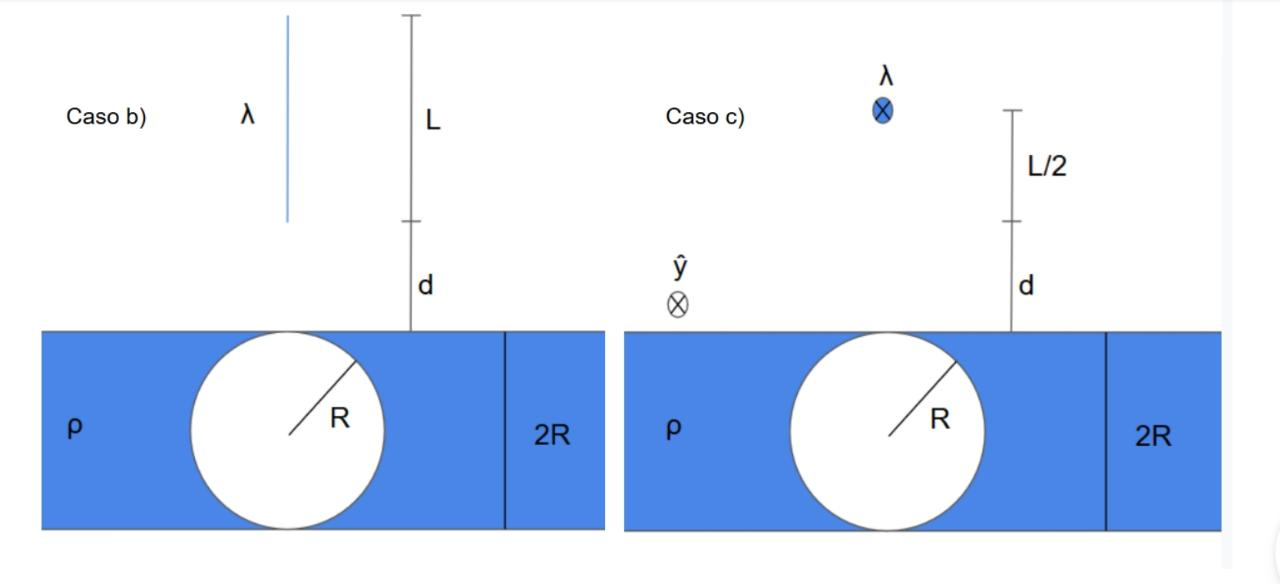
\includegraphics[width=0.9\textwidth]{Electroestática/Campo_electrico/P1 guia2 Mancilla.jpeg}
    \label{fig:P1G2M}
\end{figure}

\np
\begin{enumerate}[label=\alph*)]
    \item Si el campo eléctrico de una carga puntual fuera proporcional a $1/r^3$ en vez de $1/r^2$, ¿seguiría siendo válida la ley de Gauss? Explique su razonamiento. (Sugerencia: considere una superficie esférica centrada en una sola carga puntual).
    \item  Cierta región del espacio limitada por una superficie imaginaria cerrada no contiene carga. ¿El campo eléctrico siempre es igual a cero en todos los puntos de la superficie? Si no es así, ¿en qué circunstancias sería cero en la superficie?
    \item En cierta región del espacio, el campo eléctrico es uniforme. Use la ley de Gauss para demostrar que esa región debe ser eléctricamente neutra; es decir, la densidad volumétrica de carga $\rho$ debe ser igual a cero. Lo contrario, ¿es verdadero? Es decir, en una región del espacio donde no hay carga, ¿debe ser uniforme?
\end{enumerate}

\np
Imagine una esfera de radio R rellena con carga negativa de densidad uniforme y una carga total equivalente a la carga de dos electrones, es decir, $-2e$. En el interior de esta gelatina de carga negativa, se encuentran dos protones, cada uno de ellos de carga $e$. Asuma que, a pesar de la presencia de los protones, la distribución de carga negativa se mantiene uniforme. ¿Dónde deben ubicarse los protones de modo que la fuerza en cada uno de ellos sea nula? Para responder esta pregunta, siga estos pasos:
\begin{enumerate}[label=\alph*)]
    \item Calcule el campo eléctrico producido por los electrones.
    \item Calcule la fuerza de Coulomb neta sobre uno los protones.
    \item Determine la condición de equilibrio y concluya.
\end{enumerate}


\newpage
\subsection{Soluciones}

\sol{1}\newline\newline
$a)$ Al ser metálicas, la esfera y el cascarón son conductores.En equilibrio electrostático, la carga en la superficie interior del cascarón es $-q$ para neutralizar el campo eléctrico de la esfera (que no haya líneas de campo en el conductor) y, dado que su carga total es nula, la carga en la superficie exterior es $q$. Las densidades de carga superficial de la esfera $\sigma_S$, interior del cascarón $\sigma_I$ y exterior del cascarón $\sigma_E$ son uniformes, en el caso de $\sigma_I$ porque la esfera y el cascarón son concéntricos, y están dados por

\[\sigma_S = \frac{q}{4\pi R^2}\]
\[\sigma_I = \frac{-q}{4\pi a^2}\]
\[\sigma_E = \frac{q}{4\pi b^2}\]

$b)$ El espacio está dividido en 4 zonas: al interior de la esfera, $r<R$ (1); entre la esfera y el cascarón, $R<r<a$ (2); interior del cascarón, $a<r<b$ (3); y exterior del cascarón, $b<r$ (4). Como el sistema se compone sólo de conductores y vacío, la densidad volumétrica en todo el espacio es nula. Con esto, utilizando la ecuación de Poisson (calculada en \textbf{\ref{PoissonEsferas}}) el potencial dividido en zonas es

\begin{itemize}
    \item $V_1 = B_1 - \frac{A_1}{r}$
    \item $V_2 = B_2 - \frac{A_2}{r}$
    \item $V_3 = B_3 - \frac{A_3}{r}$
    \item $V_4 = B_4 - \frac{A_4}{r}$
\end{itemize}

Para $r\rightarrow\infty$ el potencial se anula, por lo que $B_4 = 0$, además, dado que en los conductores el potencial es constante, $A_1 = A_3 = 0$.

Los campos eléctricos en (2) y (4) poseen simetría de tipo $\Vec{E}(\Vec{r}) = E(r)\hat{r}$ (demostración en \textbf{\ref{SimetríaEsfera}}), de modo que por ley de Gauss se verifica que

\begin{itemize}
    \item $E_2 = \frac{q}{4\pi\epsilon_o r^2}$
    \item $E_4 = \frac{q}{4\pi\epsilon_o r^2}$
\end{itemize}

Utilizando $\Vec{E} = -\nabla V$ se obtiene

\[\frac{q}{4\pi\epsilon_o r^2} = -\frac{A_2}{r^2} = -\frac{A_4}{r^2}\]

\[A_2 = A_4 = -\frac{q}{4\pi\epsilon_o}\]

Finalmente, por continuidad del potencial

\[V_4(b) = V_3(b) \Rightarrow B_3 = \frac{q}{4\pi\epsilon_o b}\]
\[V_3(a) = V_2(a) \Rightarrow B_2 = \frac{q}{4\pi\epsilon_o}
\left(\frac{1}{b}-\frac{1}{a}\right)\]
\[V_2(R) = V_1(R) \Rightarrow B_1 = \frac{q}{4\pi\epsilon_o}
\left(1+\frac{1}{b}-\frac{1}{a}\right)\]

Se concluye así que

\begin{itemize}
    \item $V_1 = \frac{q}{4\pi\epsilon_o}
\left(1+\frac{1}{b}-\frac{1}{a}\right)$
    \item $V_2 = \frac{q}{4\pi\epsilon_o}\left(
    \frac{1}{r}+\frac{1}{b}-\frac{1}{a}\right)$
    \item $V_3 = \frac{q}{4\pi\epsilon_o b}$
    \item $V_4 = \frac{q}{4\pi\epsilon_o r}$
\end{itemize}
\bigbreak

$c)$ Si se baja el potencial del cascarón a 0, en consecuencia el potencial al exterior de este se anula también

\[V_3 = V_4(b) \Leftrightarrow 0 = -\frac{A_4}{b} \Leftrightarrow A_4 = 0	\Leftrightarrow V_4 = 0\]

Si $V_4 = 0$ entonces $E_4= 0$ y, por ley de Gauss, la carga total encerrada por el cascarón en nula, $\sigma_E = 0$. La carga de la esfera no se ve afectada, de modo que $E_2$ y $A_2$ se mantienen iguales, luego

\[V_2(a) = V_3 \Leftrightarrow B_2 = -\frac{q}{4\pi\epsilon_o a}\]
\[V_2(r) = \frac{q}{4\pi\epsilon_o}\left(\frac{1}{r}
-\frac{1}{a}\right)\]
\[V_1 = V_2(R) = \frac{q}{4\pi\epsilon_o}\left(\frac{1}{R}
-\frac{1}{a}\right)\]

\bigbreak

$d)$ Si $V_3 = V$ entonces

\[V_3 = V_4(b) \Leftrightarrow v = -\frac{A_4}{b} \Leftrightarrow A_4 = -Vb	\Leftrightarrow V_4 = \frac{Vb}{r}\]
\[V_2(a) = V_3 \Leftrightarrow B_2 = V-\frac{q}{4\pi\epsilon_o a}
\Leftrightarrow V_2 = V+\frac{q}{4\pi\epsilon_o}\left(\frac{1}{r}
-\frac{1}{a}\right)\]
\[\Vec{E_4}=-\nabla V_4 = \frac{Vb}{r^2}\hat{r}\]

Para $Q$ la carga total, por ley de Gauss se tiene que

\[E_4= \frac{Q}{4\pi\epsilon_o r^2} = \frac{Vb}{r^2}
\Leftrightarrow Q = 4\pi\epsilon_o Vb\]

Por lo que la carga neta del cascarón es

\[q_c = 4\pi\epsilon_o Vb - q\]

\bigbreak

$e)$ Si se conectan la esfera y el cascarón ambos conformarán un solo conductor y por lo tanto estarán a un mismo potencial. Como la diferencia de potencial es nula, el campo eléctrico en todo el espacio encerrado por el cascarón es 0. Dado que no se produce ningún cambio a la carga total, $E_4$, y por ende $V_4$, son los calculados en $b)$

\[V_1=V_2=V_3=V_4(b)=\frac{q}{4\pi\epsilon_o b}\]
\bigbreak

$f)$ La energía de los conductores desconectados es

\[U_{e1} = \frac{1}{2}(qV_1 + 0\cdot V_3) = \frac{q^2}{8\pi\epsilon_o}
\left(1+\frac{1}{b}-\frac{1}{a}\right)\]

Para los conductores conectados la energía es

\[U_{e2} = \frac{1}{2}qV_3 = \frac{q^2}{8\pi\epsilon_o b}\]

Se tiene $U_{e1} > U_{e2}$ debido a que al conectar los cascarones las cargas se desplazan a causa de un trabajo hecho por el campo, causando que la energía en el sistema disminuya.%para $U_{e1}$ a la energía de los conductores se le agrega la de la interacción entre ambos.

\bigbreak
\bigbreak

\sol{2}\newline\newline
Dado que $L \gg R_1, R_2$ el efecto que tiene cada esfera sobre el potencial de la otra puede ser despreciado. Para $q_1$ y $V_1$ la carga y potencial de la esfera de radio $R_1$, y $q_2$ y $V_2$ la carga y potencial de la esfera de radio $R_2$, se tiene

\[V_1 = \int\frac{\sigma_1}{4\pi\epsilon_o R_1}dS = 
\frac{q_1}{4\pi\epsilon_o R_1}\]

\[V_2 = \frac{q_2}{4\pi\epsilon_o R_2}\]

Como están conectadas, el potencial de las esferas debe ser igual

\[V_1 = V_2 \Leftrightarrow \frac{q_1}{R_1} = \frac{q_2}{R_2}\]

luego

\[Q = q_1 + q_2 = q_1 + \frac{R_2}{R_1}q_1 \Leftrightarrow
q_1 = \frac{R_1 Q}{R_1+R_2}\]

\[q_2 = \frac{R_2 Q}{R_1+R_2}\]

Puesto que $R_1<R_2$, la carga almacenada en la esfera de radio $R_2$ es mayor a la de radio $R_1$

\bigbreak

$b)$ El alambre es parte del conductor por lo que

\[V_{alambre} = V_1 = V_2 = \frac{Q}{4\pi\epsilon_o(R_2+R_1)}\]
\bigbreak

$c)$ La densidad de carga de las esferas es

\[\sigma_1 = \frac{q_1}{4\pi R_1^2} =
\frac{Q}{4\pi R_1(R_1+R_2)}\]
\[\sigma_2 = \frac{q_2}{4\pi R_2^2} =
\frac{Q}{4\pi R_2(R_1+R_2)}\]

Como $R_2 > R_1$, $\sigma_2 < \sigma_1$. El campo eléctrico en las superficies es

\[\Vec{E_1}=\frac{\sigma_1}{\epsilon_o}\hat{r_1}\]
\[\Vec{E_2}=\frac{\sigma_2}{\epsilon_o}\hat{r_2}\]

Donde $\hat{r_i}$ es el vector unitario $\hat{r}$ de las coordenadas esféricas respecto al centro de la esfera de radio $R_i$.
\bigbreak
\bigbreak

\sol{3}\newline\newline
 Usando coordenadas esféricas con origen en el centro de las capas, el espacio se divide en 4 zonas: $r < a$ (1), $a<r<2a$ (2), $2a<r<3a$ (3) y $3a<r$ (4). Las esferas presentan simetría (demostración en \textbf{\ref{SimetríaEsfera}}), por lo que se puede calcular su campo eléctrico con ley de Gauss. Como el sistema comprende sólo conductores y vacío $\rho = 0$ en todo el espacio. De la ecuación de Poisson (resuelta en \ref{PoissonEsferas}) se desprende que en cada zona el potencial es de forma
\[V = B-\frac{A}{r}\]


\begin{enumerate}[label=\alph*)]
    \item Como en (1) no hay carga el campo es nulo
    \[E_1 = 0\]
    \item En (2) la carga encerrada es $Q_{in}$, por lo que el campo eléctrico es
    \[\Vec{E_2} = \frac{Q_{in}}{4\pi\epsilon_o r^2}\hat{r}\]
    \item En (3) la carga encerrada es $Q_{in}+Q$, por lo que el campo eléctrico es
    \[\Vec{E_2} = \frac{Q_{in}+Q}{4\pi\epsilon_o r^2}\hat{r}\]
    \item Para que no haya campo eléctrico al interior del conductor exterior se debe cumplir que $Q_{out} = -(Q+Q_{in})$. Como en el infinito el potencial se anula, en (4) $B=0$ y $V = -\frac{A}{r}$. Igualando $V$ a 0 en $3a$ se obtiene que $A=V=0$ y en concecuencia
    \[E_4 = 0\]


    \item Para $V_2$ el potencial en (2), se verifica que

    \begin{equation}
    \begin{split}
        V_2(r) & = V_2(r) - V_2(a)\\
        & = -\int^r_a\Vec{E_2}\cdot d\Vec{r'}\\
       & = -\int^r_a\frac{Q_{in}}{4\pi\epsilon_o {r'}^2}\,dr'\\
       & = \frac{Q_{in}}{4\pi\epsilon_o r} - \frac{Q_{in}}{4\pi\epsilon_o a}\\
    \end{split}
    \nonumber
    \end{equation}
    Con lo que el potencial en la capa intermedia es

    \[V_2(2a) = -\frac{Q_{in}}{8\pi\epsilon_o a}\]
    \medbreak
    Para $V_3$ el potencial en (3), se verifica que

    \begin{equation}
    \begin{split}
      V_3(r) & = V_3(r) - V_3(3a)\\
      & = -\int^r_{3a}\Vec{E_3}\cdot d\Vec{r'}\\
      & = -\int^r_{3a}\frac{Q_{in}+Q}{4\pi\epsilon_o {r'}^2}\,dr'\\
      & = \frac{Q_{in}+Q}{4\pi\epsilon_o r} - \frac{Q_{in}+Q}{12\pi\epsilon_o a}\\
    \end{split}
    \nonumber
    \end{equation}
    Con lo que el potencial en la capa intermedia es

    \[V_3(2a) = \frac{Q_{in}+Q}{24\pi\epsilon_o a}\]
    \medbreak
    \item Como $V_2(2a)=V_3(2a)$, se tiene que

    \[\frac{Q_{in}+Q}{24\pi\epsilon_o a} = -\frac{Q_{in}}{8\pi\epsilon_o a}\]
    \[\implies Q_{in}=-\frac{1}{4}Q\]
    
    \medbreak
    \item Puesto que las capas exterior e interior están a igual potencial se las puede tomar como un solo conductor de carga $Q_{in} + Q_{out} = -Q$, formando un condensador con la capa intermedia. La capacitancia del sistema está dada por
    
    
    \[C = \frac{Q}{\Delta V} = 32\pi\epsilon_o a\]
    
    Esto también se puede ver como si se tuvieran dos condensadores en paralelo, uno con carga $Q_{in}$ y otro con carga $Q_{out}$ y misma diferencia de potencial $V(2a)$. Al estar en paralelos su capacitancia equivalente sería la suma de las capacitancias individuales, dando el resultado anterior.
    
    La razón de que pueden verse como condensadores en paralelo yace en que poseen el mismo potencial en ambos extremos, en uno están a potencial $V=0$ y en el otro a potencial $V = V(2a)$. En la siguiente imagen se visualiza de manera circuital
    
    \begin{figure}[H]
        \centering
        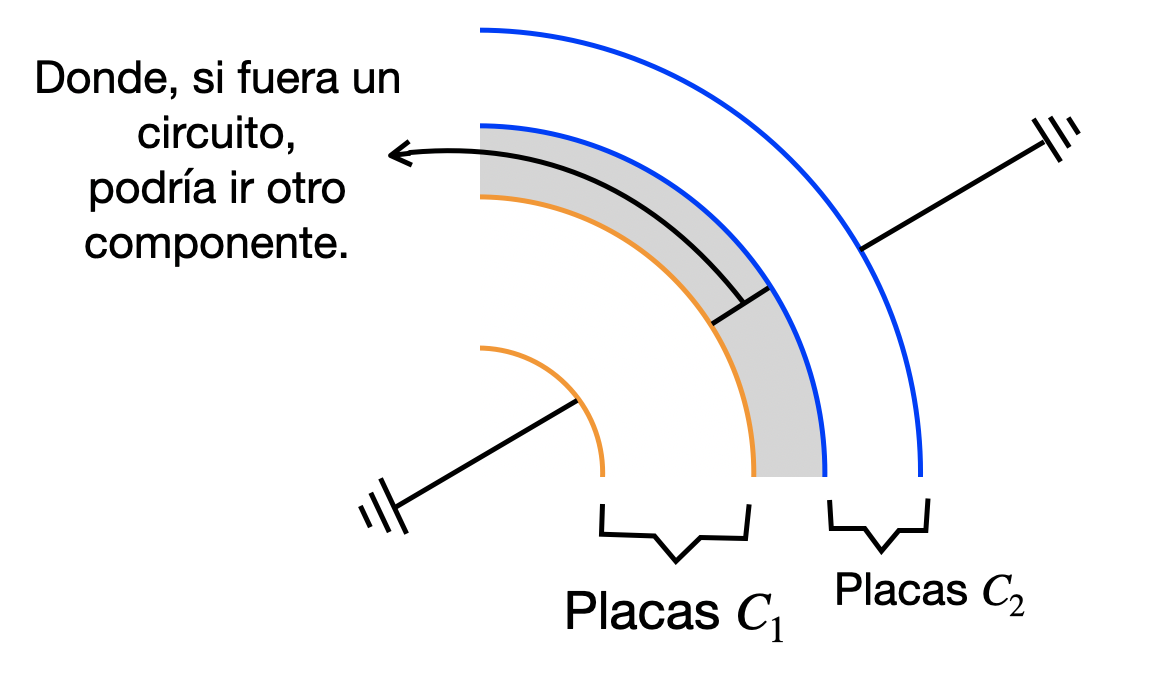
\includegraphics[width=0.5\textwidth]{Electroestática/conductores/P3IG.png}
    \end{figure}
    
    En la figura anterior el conductor de radio $a$ es el inferior izquierdo, el conductor de radio $2a$ está representado por el conductor 'con anchura' de color gris, y el conductor de radio $3a$ es el superior derecho. Las conexiones con 3 líneas representan conexiones a tierra. Y los condensadores son representados el primero con color amarillo-naranjo y el segundo con color azul. 
    
    \medbreak
    \item El sistema está compuesto por 3 conductores y 2 condensadores, como las capas interna y externa tienen potencial nulo, la energía queda dada sólo por la capa intermedia

    \[U_e = \frac{1}{2}V_2(2a) = \frac{1}{8}\frac{Q^2}{8\pi\epsilon_o a}\]
    
    Esto es equivalente a calcular la capacitancia de un condensador equivalente y, haciendo uso de $V(2a)$, obtener la energía potencial con
    $U_e = \frac{1}{2}C\Delta V^2$. 

\end{enumerate}
\bigbreak
\bigbreak
\sol{4}\newline
% Podriamos especificar la alineación de las placas y agregar imagen

\begin{enumerate}[label=\alph*)]
    %a
    \item Como las dimensiones laterales de las placas son mucho más grandes que $x$, se puede aproximar el campo eléctrico de una de las placas al de un plano infinito

    \[\Vec{E} = \frac{Q}{2A\epsilon_o}\hat{x}\]

    ubicando el origen en la placa de carga $Q$, el trabajo par desplazar la placa de carga $-Q$ en $\Delta x$ es

    \begin{equation}
        \begin{split}
            W_{ext} &= Q\int^{x+\Delta x}_x \Vec{E}\cdot d\Vec{r}\\
            & = Q\int^{x+\Delta x}_x\frac{Q}{2A\epsilon_o}\,dr\\
            & = \frac{Q^2}{2A\epsilon_o}\Delta x\\
        \end{split}
        \nonumber
    \end{equation}
    \medbreak
%b
    \item Por teorema de trabajo-energía, se cumple que la diferencia de energía potencial es igual al trabajo hecho por la fuerza externa, por lo que

    \[\Delta U_e = W = \frac{Q^2}{2A\epsilon_o}\Delta x\]
    Notemos que al ser el trabajo positivo, la fuerza externa está inyectando energía al sistema, por lo que se tiene que no se conserva la energía del sistema al aumentar la separación entre las placas por un $\Delta x$
    
    La energía potencial del sistema también se puede calcular haciendo uso del condensador, donde $U_e = \frac{1}{2}Q\Delta V = \frac{Q^2}{2C}$. Como se tiene que la carga de las placas no cambia, entonces se tiene que $C$ y $\Delta V$ han de cambiar. En específico, como se separan las placas $C$ pasa a ser $\frac{\epsilon_o A}{x+\Delta x}$ (calculado en \ref{C:placas}).
%c Aux_5 Daniela Mancilla Otoño 2020
    \item Siguiendo la idea del párrafo anterior, si es que al realizar trabajo cambia la energía del sistema, lo que implica un cambio en el condensador, (carga o diferencia de potencial) entonces al mantener la batería conectada se mantendrá la diferencia de potencial igual. Con esto en mente, entonces será necesario que la carga del condensador cambie.
    
    \begin{equation}
    \begin{split}
        W_{ext} &= \int^{x+\Delta x}_x Q\Vec{E}\cdot d\Vec{r}\\
        & = \int^{x+\Delta x}_x \frac{Q^2}{2A\epsilon_o}\,dr\\
        & = \int^{x+\Delta x}_x
        \frac{(CV_o)^2}{2A\epsilon_o}\,dr\\
        & = \int^{x+\Delta x}_x
        \frac{\epsilon_o AV_o^2}{2r^2}\,dr\\
        &=\frac{\epsilon_o AV_o^2}{2}\left(
        -\frac{1}{x+\Delta x}+\frac{1}{x}\right)\\
        &=\frac{\epsilon_o AV_o^2\Delta x}{2x(x+\Delta x)}
    \end{split}
    \nonumber
    \end{equation} 
    
    \medbreak

%d
    \item La energía potencial eléctrica inicial es
    
    \[U_i = \frac{1}{2}C_iV_o^2 = \frac{\epsilon_o A}{2x}V_o^2\]
    
    la energía potencial final es
    
    \[U_f = \frac{1}{2}C_fV_o^2 = 
    \frac{\epsilon_o A}{2(x+\Delta x)}V_o^2\]
    
    de modo que
    
    \[\Delta U = U_f-U_i = -\frac{\epsilon_o AV_o^2\Delta x}{2x(x+\Delta x)}\]
    
    % Hay que mostrar que la energía que se conserva

\end{enumerate}

\bigbreak
\bigbreak

\sol{5}\newline

\begin{enumerate}[label=\alph*)]
    \item El campo eléctrico en todo el espacio puede ser obtenido haciendo uso de la Ley de Gauss y de la definición de campo eléctrico, debido a lo que será pedido en los siguientes incisos solo será calculado en el caso $\rho > a$ y $\abs{z} < L/2$. Donde se están usando coordenadas cilíndricas y el centro del cilindro como eje.\\
    
    Partamos calculando la densidad superficial de carga, la densidad de carga es superficial a causa de que estamos frente a un conductor que no puede tener campo eléctrico interno, con esto tenemos que 
    \[\sigma = \frac{Q}{2\pi aL}\]
    A causa de que está solo en el manto y el área del manto es $2\pi aL$.\\
    
    Haciendo uso de la Ley de Gauss y sabiendo que por simetría (\ref{SimetríaCilindrosInf}) hay solo campo en la dirección $\hat{\rho}$, establecemos un cilindro más grande superpuesto con el original, de radio $\rho$ y altura $h$, con esto
    %no tiene que ser infinito?, no también el largo(altura) puede ser mucha mayor al radio
    \begin{equation}
        \begin{split}
            &\oint_{Manto} \Vec{E}\cdot d\Vec{S} = \frac{Q_{enc}}{\epsilon_0}\\
            \implies &\int E(\rho)dS = \frac{\sigma 2\pi a h}{\epsilon_0}\\
            \implies &E(\rho) \int dS = \frac{\sigma 2\pi a h}{\epsilon_0}\\
            \implies &E(\rho) 2 \pi \rho h = \frac{\sigma 2\pi a h}{\epsilon_0}\\
            \implies &E(\rho) = \frac{\sigma a}{\epsilon_0 \rho}\\
            \therefore \quad &\Vec{E}(\rho) = \frac{\sigma a}{\epsilon_0 \rho}\hat{\rho}
        \end{split}
        \nonumber 
    \end{equation}
    
    \item Sea $\sigma_+$ la densidad superficial del manto del cilindro de radio $a_1$ y $\sigma_-$ la densidad superficial del manto del cilindro de radio $a_2$, tenemos que el campo eléctrico de cada cilindro será
    
    \[\Vec{E}_{a_1} = \frac{\sigma_+ a_1}{\epsilon_0 \rho}\hat{\rho}\]
    \[\Vec{E}_{a_2} = \frac{\sigma_- a_2}{\epsilon_0 \rho}\hat{\rho'}\]
    
    Si calculamos el campo en $P$ debemos sumar ambos campos, y se tiene que $\hat{\rho'} = - \hat{\rho}$, ya que están centrados en distintos ejes los campos, y en $P$ las direcciones son justo contrarias, así
    
    \[\Vec{E}_{\text{en P}} = \left( \frac{\sigma_+ a_1}{\epsilon_0 r} - \frac{\sigma_- a_2}{\epsilon_0 (d-r)} \right)\hat{\rho}\]
    
    \item Para calcular la diferencia de potencial calculamos $V(a_1) - V(d - a_2)$ por definición,
    
    \begin{equation}
        \begin{split}
            V(a_1) - V(d - a_2) &= -\int_{d-a_2}^{a_1}\left[ \frac{\sigma_+ a_1}{\epsilon_0 r} - \frac{\sigma_- a_2}{\epsilon_0 (d-r)} \right]dr\\
            &= -\left.\left[ \frac{\sigma_+ a_1}{\epsilon_0}\ln{(r)} + \frac{\sigma_- a_2}{\epsilon_0}\ln{(d-r)} \right]\right\rvert_{d-a_2}^{a_1}\\
            &\vdots \quad\\ 
            &\approx -\left[ \frac{\sigma_+}{\epsilon_0}a_1\ln{\left( \frac{a_1}{d} \right)} - \frac{\sigma_-}{\epsilon_0}a_2\ln{\left( \frac{a_2}{d} \right)} \right]\\
            \text{Donde en } \vdots \text{ se usó que } &d-a_1 \approx d\text{ y } d-a_2 \approx d\text{, al ser }d \gg a_1\text{ y } d \gg a_2\\
        \end{split}
        \nonumber
    \end{equation}
    
    Reemplazamos $\sigma_+ = Q/(2\pi La_1)$ y $\sigma_- = -Q/(2\pi La_2)$, y nos queda
    
    \begin{equation}
        \begin{split}
            \Delta V &= -\left[ \frac{Q}{2 \pi L\epsilon_0}\ln{\left( \frac{a_1}{d} \right)} + \frac{Q}{2 \pi L\epsilon_0}\ln{\left( \frac{a_2}{d} \right)} \right]\\
            &=\frac{Q}{2 \pi L \epsilon_0}\ln{\left( \frac{d^2}{a_1a_2} \right)}\\
            &=\frac{Q}{\pi L \epsilon_0}\ln{\left( \frac{d}{\sqrt{a_1a_2}} \right)}
        \end{split}
        \nonumber
    \end{equation}
    
    Lo que nos da que la capacitancia del sistema es
    \[C_{tot} \approx \frac{Q}{\Delta V} = \frac{\pi \epsilon_0 L}{\ln{\left( \frac{d}{\sqrt{a_1a_2}} \right)}}\]
    
    \item Como se tiene que nos piden la capacitancia por unidad de largo debemos dividir la capacitancia encontrada por $L$, así
    \[C \approx \frac{\pi \epsilon_0}{\ln{\left( \frac{d}{\sqrt{a_1a_2}} \right)}}\]
    
    \item Está situación es similar a la presentada en el problema 7.2, por lo que las cargas se distribuirían a través de los cilindros dependiendo de las razones entre sus radios, y el potencial se volvería el mismo para ambos.
    
\end{enumerate}

\sol{6}\newline

\begin{enumerate}[label=\alph*)]
    \item Digamos que la capa del radio interno tiene una carga $-Q$ en su cara exterior, y la capa externa una carga $Q$ en su cara interior. Así queda la configuración como en la siguiente imagen
    \begin{figure}[H]
        \centering
        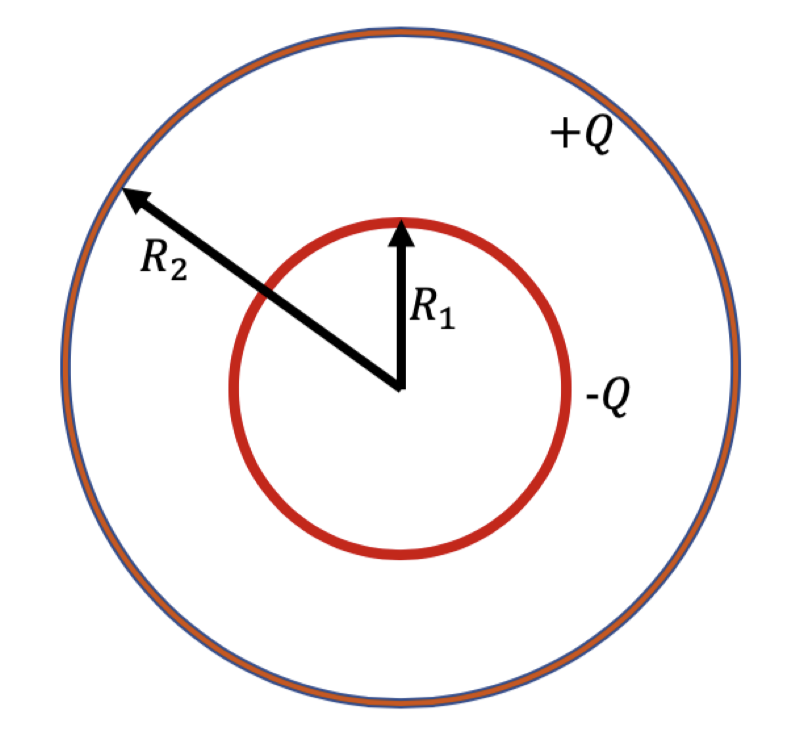
\includegraphics[width=0.47\textwidth]{Electroestática/conductores/P6IA.png}
        \label{fig:sol_6_conduc}
    \end{figure}
    
    Para calcular la capacitancia calculemos la diferencia de potencial entre ambas caras, para esto calculemos el campo eléctrico e integramos de $R_1$ a $R_2$.\\
    
    Usando Ley de Gauss y una superficie Gaussiana de largo $L$ y radio $\rho$, con $R_1 < \rho < R_2$,
    \[\oint_{Manto} \Vec{E}\cdot d\Vec{S} = \frac{Q_{enc}}{\epsilon_0}\]
    \[\implies E(\rho) = \frac{-Q}{2 \pi L \epsilon_0 \rho}\]
    Ahora calculamos la diferencia de potencial,
    \[\Delta V = V(R_2) - V(R_1) =-\int_{R_1}^{R_2}\frac{-Q}{2 \pi L \epsilon_0 \rho}d\rho = \frac{Q}{2\pi L \epsilon_0}\ln{\left( \frac{R_2}{R_1} \right)}\]
    Ahora usando $C = Q/\Delta V$ podemos obtener la capacitancia del sistema
    \[C = \frac{Q}{\Delta V} = \frac{2\pi L \epsilon_0}{\ln{\left( \frac{R_2}{R_1} \right)}}\]
    \text{ }\\     
    % Problema 2 Aux 5 D. Mancilla Otoño2020 (Pauta en Ucursos)
    
    \item \textbf{(Sin valores actualmente)} El nuevo condensador es como el mostrado a continuación
    \begin{figure}[H]
        \centering
        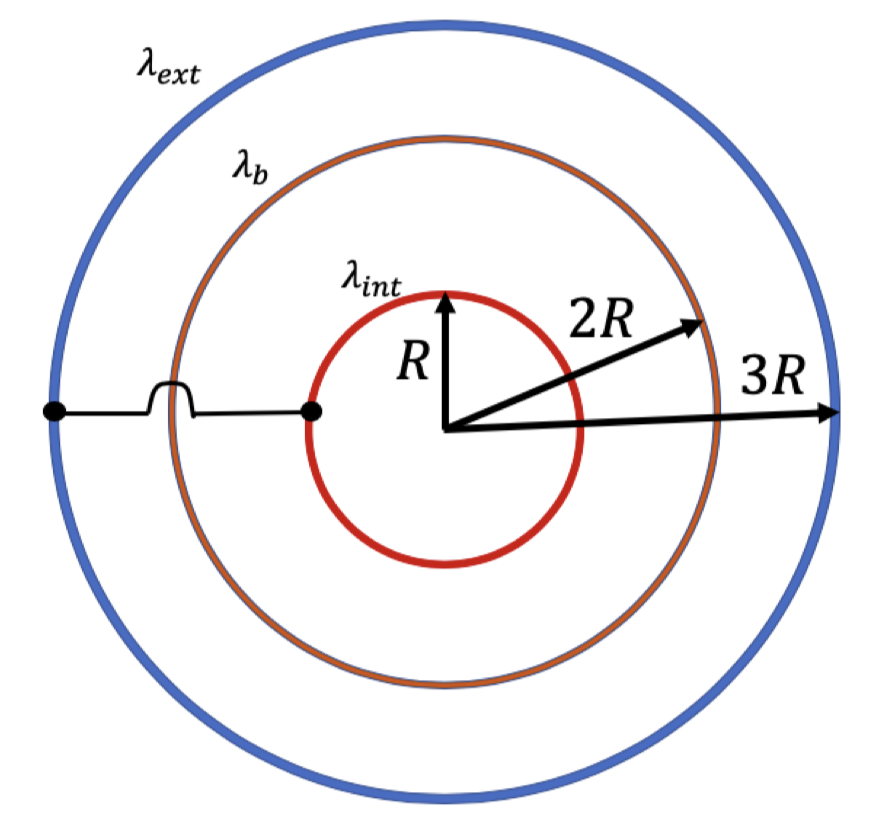
\includegraphics[width=0.47\textwidth]{Electroestática/conductores/P6IB.png}
    \end{figure}
    % Completar respuestas con desarrollo y resultados
    Como se tiene que la capa de radio $R$ y la de radio $3R$ están conectadas entonces sus potenciales son iguales, sabiendo esto y con la Ley de Gauss se puede calcular el campo eléctrico y obtener expresiones para los voltajes. Y usando $V(R) - V(2R) = V(3R) - V(2R)$ se puede despejar $\lambda_{int}$. Luego usando que son conductores y comienzan neutrales se tiene $0 = \lambda_{ext} + \lambda_{int} + \lambda_b$, y se puede obtener el valor de $\lambda_{ext}$
    % Completar respuestas con desarrollo y resultados    
    \item Para despejar la capacitancia se ocupa la relación entre energía potencial eléctrica y capacitancia, y además se despeja usando la definición que la relaciona con el voltaje.
    % (Copiado del aux)
    \item Las cargas ($\lambda_{int}, \lambda_{ext} $ y $ \lambda_b$) permanecen donde se encontraban. Con respecto a $\lambda_{nuevo}$, se distribuirá de manera uniforme en la superficie exterior ($r=3R$).
    
    
\end{enumerate}
\newpage

\end{document}